%!TEX root = ../main.tex
\chapter{Le onde}

Equazioni delle onde
\begin{itemize}
    \item $n=1$, $\displaystyle u_{tt} -c^{2} u_{xx} =f$.

          Onde trasversali di una corda di piccola ampiezza.
    \item $\displaystyle n=2,3$, $\displaystyle u_{tt} -c^{2} \Delta u=f$.

          Onde d'acqua \textit{lineari}, acustiche, elettromagnetiche nel vuoto.
\end{itemize}

\section{Equazione della corda vibrante in \texorpdfstring{$n=1$}{n=1}}

Ricaviamo ora l'equazione della corda vibrante unidimensionale (tipicamente corda di violino o chitarra). Lavoriamo sotto le seguenti ipotesi:
\begin{enumerate}
    \item Vibrazioni della corda \textbf{piccole} (relativamente alla lunghezza): i cambiamenti del profilo della corda rispetto all'orizzontale sono \textit{piccoli.}
    \item Lo spostamento di ogni punto della corda è \textbf{verticale.}
    \item Lo spostamento verticale $u$ di un punto dipende solo dalla sua posizione sulla corda $x$ e dal tempo $t$. Quindi
          \begin{equation*}
              u=u(x,t)
          \end{equation*}

          e dalla prima ipotesi deduciamo $\displaystyle | u_{x}(x,t)| \ll 1$.
    \item La corda è \textbf{perfettamente flessibile}: non offre resistenza alla flessione. L'unica forza agente sulla corda è la tensione $T$, diretta tangenzialmente, di intensità $\displaystyle \tau \ (=| T|)$.
    \item Gli attriti sono \textbf{trascurabili.}
\end{enumerate}

\textbf{Leggi generali}
\begin{itemize}
    \item Conservazione della massa.
    \item Bilancio del momento lineare (ovvero 2a legge della dinamica).
\end{itemize}

Sia $\displaystyle \rho =\rho (x,t)$ la densità lineare di massa al tempo $t$ e $\displaystyle \rho _{0} =\rho _{0}(x)$ la densità a riposo. Prendiamo in esame un tratto di corda corrispondente ad un intervallo arbitrario $\displaystyle [ x,x+\Delta x]$ e indichiamo con $\displaystyle \Delta s$ l'elemento di lunghezza corrispondente, al tempo $t$. La legge di conservazione della massa impone
\begin{equation*}
    \rho _{0}(x) \Delta x=\rho (x,t) \Delta s,\ t\geq 0
\end{equation*}
L'equazione del bilancio del momento si ricava uguagliando la forza totale agente sul generico tratto considerato al tasso di variazione del momento lineare. Poiché il moto è verticale, le componenti orizzontali delle forze devono bilanciarsi: $R_{x}=0$. Indicando con $\displaystyle \tau (x,t)$ la tensione (scalare, ma non adimensionale) in $x$

\begin{figure}[htpb]
    \centering


    \tikzset{every picture/.style={line width=0.75pt}} %set default line width to 0.75pt        

    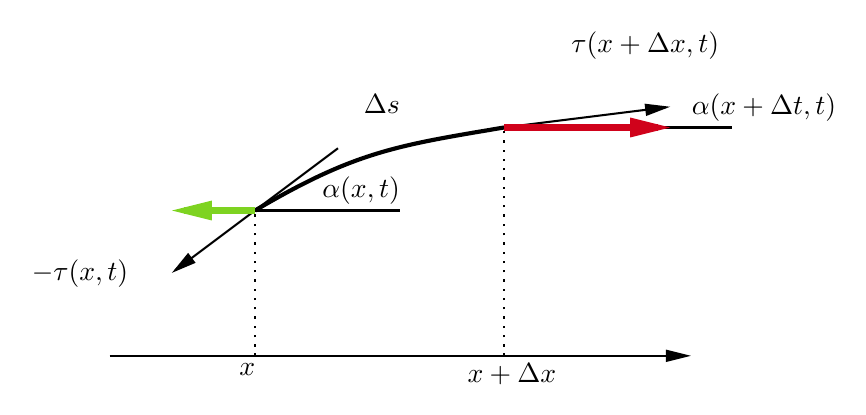
\begin{tikzpicture}[x=0.75pt,y=0.75pt,yscale=-1,xscale=1]
        %uncomment if require: \path (0,229); %set diagram left start at 0, and has height of 229

        %Straight Lines [id:da6928670195910238] 
        \draw    (120,180) -- (398,180) ;
        \draw [shift={(400,180)}, rotate = 180] [fill={rgb, 255:red, 0; green, 0; blue, 0 }  ][line width=0.08]  [draw opacity=0] (12,-3) -- (0,0) -- (12,3) -- cycle    ;
        %Straight Lines [id:da6098006131722913] 
        \draw  [dash pattern={on 0.84pt off 2.51pt}]  (190,180) -- (190,110) ;
        %Straight Lines [id:da4857013571855955] 
        \draw  [dash pattern={on 0.84pt off 2.51pt}]  (310,180) -- (310,70) ;
        %Curve Lines [id:da45458961680801546] 
        \draw [line width=1.5]    (190,110) .. controls (238,81.7) and (258,78.7) .. (310,70) ;
        %Straight Lines [id:da8988348549437535] 
        \draw    (190,110) -- (151.6,138.8) ;
        \draw [shift={(150,140)}, rotate = 323.13] [fill={rgb, 255:red, 0; green, 0; blue, 0 }  ][line width=0.08]  [draw opacity=0] (12,-3) -- (0,0) -- (12,3) -- cycle    ;
        %Straight Lines [id:da8586274723376333] 
        \draw    (310,70) -- (388.02,60.25) ;
        \draw [shift={(390,60)}, rotate = 532.87] [fill={rgb, 255:red, 0; green, 0; blue, 0 }  ][line width=0.08]  [draw opacity=0] (12,-3) -- (0,0) -- (12,3) -- cycle    ;
        %Straight Lines [id:da16414524179036505] 
        \draw    (190,110) -- (260,110) ;
        %Straight Lines [id:da5815732755450487] 
        \draw    (190,110) -- (230,80) ;
        %Straight Lines [id:da18438798249466148] 
        \draw    (310,70) -- (420,70) ;
        %Straight Lines [id:da613841499053857] 
        \draw [color={rgb, 255:red, 126; green, 211; blue, 33 }  ,draw opacity=1 ][line width=2.25]    (190,110) -- (156,110) ;
        \draw [shift={(150,110)}, rotate = 360] [fill={rgb, 255:red, 126; green, 211; blue, 33 }  ,fill opacity=1 ][line width=0.08]  [draw opacity=0] (19.2,-4.8) -- (0,0) -- (19.2,4.8) -- cycle    ;
        %Straight Lines [id:da869175453205467] 
        \draw [color={rgb, 255:red, 208; green, 2; blue, 27 }  ,draw opacity=1 ][line width=2.25]    (310,70) -- (384,70) ;
        \draw [shift={(390,70)}, rotate = 180] [fill={rgb, 255:red, 208; green, 2; blue, 27 }  ,fill opacity=1 ][line width=0.08]  [draw opacity=0] (19.2,-4.8) -- (0,0) -- (19.2,4.8) -- cycle    ;

        % Text Node
        \draw (341,22.4) node [anchor=north west][inner sep=0.75pt]    {$\tau (x+\Delta x,t)$};
        % Text Node
        \draw (81,132.4) node [anchor=north west][inner sep=0.75pt]    {$-\tau (x,t)$};
        % Text Node
        \draw (291,182.4) node [anchor=north west][inner sep=0.75pt]    {$x+\Delta x$};
        % Text Node
        \draw (181,182.4) node [anchor=north west][inner sep=0.75pt]    {$x$};
        % Text Node
        \draw (221,92.4) node [anchor=north west][inner sep=0.75pt]    {$\alpha (x,t)$};
        % Text Node
        \draw (399,52.4) node [anchor=north west][inner sep=0.75pt]    {$\alpha (x+\Delta t,t)$};
        % Text Node
        \draw (241,52.4) node [anchor=north west][inner sep=0.75pt]    {$\Delta s$};

    \end{tikzpicture}
    \caption{Tensione agli estremi di un piccolo arco di corda.}
\end{figure}
\FloatBarrier

%\fg[Tensione agli estremi di un piccolo arco di corda]{0.6}{onde-tensione-arco}

\begin{equation*}
    0=R_{x} =\textcolor[rgb]{0.82,0.01,0.11}{\tau (x+\Delta x,t)\cos \alpha (x+\Delta x,t)} -\textcolor[rgb]{0.49,0.83,0.13}{\tau (x,t)\cos \alpha (x,t)}
\end{equation*}
Dividendo per $\displaystyle \Delta x$ e facendo il limite per $\displaystyle \Delta x\rightarrow 0$ diventa una derivata
\begin{equation*}
    \frac{\partial }{\partial x}[ \tau (x,t)\cos \alpha (x,t)] =0
\end{equation*}
Questa è la tensione orizzontale, e risulta costante per $x$ fissato
\begin{equation*}
    \tau _{\text{oriz}}(x,t) =\tau (x,t)\cos \alpha (x,t) =\tau _{0}(t)
\end{equation*}
dove $\displaystyle \tau _{0}(t) \geq 0$ perché un'intensità.

Calcoliamo le componenti verticali delle forze agenti sul tratto considerato
\begin{equation*}
    \tau _{\text{vert}}(x,t) =\tau (x,t)\sin \alpha (x,t) =\underbrace{\tau (x,t)\cos \alpha (x,t)}_{\tau _{0}(t)}\underbrace{\tan \alpha (x,t)}_{u_{x}(x,t)} =\tau _{0}(t) u_{x}(x,t)
\end{equation*}
Dunque la risultante verticale è
\begin{align*}
    \text{tensioni} & =\tau _{\text{vert}}(x+\Delta x,t) -\tau _{\text{vert}}(x,t)                     \\
                    & =\textcolor[rgb]{0.29,0.56,0.89}{\tau _{0}(t)[ u_{x}(x+\Delta x,t) -u_{x}(x,t)}]
\end{align*}
Consideriamo ora le forze esterne di \textbf{volume} \textbf{verticali} come il peso o carichi esterni. Sia $\displaystyle f=f(x,t)$ l'intensità per unità di massa della risultante di tali forze. Per la legge di conservazione della massa, la forza agente sul tratto di corda esaminato è
\begin{align*}
    \text{forze di volume} & =\rho (x,t) f(x,t) \Delta s                                    \\
                           & =\textcolor[rgb]{0.96,0.65,0.14}{\rho _{0}(x) f(x,t) \Delta x}
\end{align*}
Applichiamo ora la seconda legge di Newton: le forze agenti sono
\begin{align*}
    \text{forze risultanti} & =\text{tensioni} +\text{forze di volume}
\end{align*}
mentre
\begin{align*}
    \text{massa} \cdotp \text{accelerazione} & =\rho (x) u_{tt} \Delta s                                   \\
                                             & =\textcolor[rgb]{0.56,0.07,1}{\rho _{0}(x) u_{tt} \Delta x}
\end{align*}
osservando che $\displaystyle u_{tt}$ è l'accelerazione scalare.

Quindi
\begin{equation*}
    \text{massa} \cdotp \text{accelerazione} =\text{forze risultanti}
\end{equation*}
da cui si ricava
\begin{equation*}
    \textcolor[rgb]{0.56,0.07,1}{\rho _{0}(x) u_{tt} \Delta x} =\textcolor[rgb]{0.29,0.56,0.89}{\tau _{0}(t)[u_{x}(x+\Delta x,t)-u_{x}(x,t)}] +\textcolor[rgb]{0.96,0.65,0.14}{\rho _{0}(x)f(x,t)\Delta x}
\end{equation*}
dividendo per $\displaystyle \Delta x$ e passando al limite per $\displaystyle \Delta x\rightarrow 0$ ottengo
\begin{equation*}
    \rho _{0}(x) u_{tt} =\tau _{0}(t) u_{xx} +\rho _{0} (x)f(x,t)
\end{equation*}
Da cui, definita
\begin{equation*}
    c^{2} =\frac{\tau _{0}(t)}{\rho _{0}(x)}
\end{equation*}
arrivo all'equazione della corda vibrante
\begin{equation}
    \boxed{u_{tt} -c^{2} u_{xx} =f(x,t)}
\end{equation}
\begin{nb}
    Le dimensioni di $\displaystyle c^{2}$ e $c$ sono
    \begin{equation*}
        [ c]^{2} =\frac{[ F]}{[ M] /[ L]} =\frac{\cancel{[ M]}\frac{[ L]}{[ T]^{2}}}{\cancel{[ M]} /[ L]} =\frac{[ L]^{2}}{[ T]^{2}} \ \ \Rightarrow \ \ [ c] =\frac{[ L]}{[ T]}
    \end{equation*}
    quelle di una velocità
\end{nb}
\begin{nb}
    Se la corda è omogenea
    \begin{equation*}
        \rho _{0}(x) =\rho _{0} \ \text{costante}
    \end{equation*}
    Se la corda è perfettamente elastica
    \begin{equation*}
        \tau _{0}(t) =\tau _{0} \ \text{costante}
    \end{equation*}
    Allora sotto entrambe le ipotesi
    \begin{equation*}
        c^{2} =\frac{\tau _{0}(t)}{\rho _{0}(x)} \ \text{costante}
    \end{equation*}
    D'ora in poi lavoreremo sempre sotto queste ipotesi.
\end{nb}
\section{Energia}

Consideriamo una corda a riposo (al tempo $t=0$) in posizione orizzontale sull'asse $x$, occupante un segmento $\displaystyle [ 0,L]$. Essendo $\displaystyle u_{t}(x,t)$ la velocità di vibrazione verticale della particella di corda in $x$, l'\textbf{energia cinetica totale }durante la vibrazione è
\begin{equation}
    E_{\text{cin}}(t) =\frac{1}{2}\int ^{L}_{0} \rho _{0} u^{2}_{t} \dx
\end{equation}
La corda immagazzina anche \textbf{energia potenziale} dovuta al lavoro delle forze elastiche. In un elemento di corda con lunghezza a riposo $\dx$, l'allungamento dovuto alle forze elastiche è pari a

\begin{figure}[htpb]
    \centering
    \tikzset{every picture/.style={line width=0.75pt}} %set default line width to 0.75pt        

    \begin{tikzpicture}[x=0.75pt,y=0.75pt,yscale=-1,xscale=1]
        %uncomment if require: \path (0,82); %set diagram left start at 0, and has height of 82

        %Straight Lines [id:da326126699745247] 
        \draw    (98,60.73) -- (353,60.73) ;
        \draw [shift={(355,60.73)}, rotate = 180] [fill={rgb, 255:red, 0; green, 0; blue, 0 }  ][line width=0.08]  [draw opacity=0] (12,-3) -- (0,0) -- (12,3) -- cycle    ;
        %Straight Lines [id:da8517694361355719] 
        \draw [color={rgb, 255:red, 208; green, 2; blue, 27 }  ,draw opacity=1 ] [dash pattern={on 0.84pt off 2.51pt}]  (190.83,33.25) -- (190.83,61.25) ;
        %Straight Lines [id:da9078704697007101] 
        \draw [color={rgb, 255:red, 208; green, 2; blue, 27 }  ,draw opacity=1 ] [dash pattern={on 0.84pt off 2.51pt}]  (260.83,14.75) -- (260.83,61.5) ;
        %Straight Lines [id:da43540991422442943] 
        \draw [color={rgb, 255:red, 208; green, 2; blue, 27 }  ,draw opacity=1 ]   (190.83,33.25) -- (260.83,14.75) ;

        % Text Node
        \draw (107.83,66.4) node [anchor=north west][inner sep=0.75pt]  [font=\scriptsize]  {$0$};
        % Text Node
        \draw (183.83,65.9) node [anchor=north west][inner sep=0.75pt]  [font=\scriptsize]  {$x$};
        % Text Node
        \draw (241.33,64.4) node [anchor=north west][inner sep=0.75pt]  [font=\scriptsize]  {$x+\dx$};
        % Text Node
        \draw (329.33,65.9) node [anchor=north west][inner sep=0.75pt]  [font=\scriptsize]  {$L$};
        % Text Node
        \draw (192.83,14.4) node [anchor=north west][inner sep=0.75pt]  [font=\scriptsize,color={rgb, 255:red, 208; green, 2; blue, 27 }  ,opacity=1 ]  {$\ds$};

    \end{tikzpicture}
\end{figure}
\FloatBarrier

\begin{equation*}
    \text{allungamento} = \ds-\dx=\sqrt{1+u^{2}_{x}} \dx-\dx=\underbrace{\left(\sqrt{1+u^{2}_{x}} -1\right)}_{|u_{x} |\ll 1} \dx\cong\footnote{Per $\varepsilon \ll 1$, $\sqrt{1+\varepsilon}\approx 1+\varepsilon/2 $} \frac{1}{2} u^{2}_{x} \dx
\end{equation*}
Quindi il lavoro compiuto da tali forze elastiche\footnote{Stiamo trattando piccole vibrazioni, $\displaystyle \tau $ non dipende da $x$.} è
\begin{equation*}
    dW= \text{forza}\cdot\text{allungamento}= \frac{1}{2} \tau _{0} u^{2}_{x} \dx
\end{equation*}
Sommando i contributi di tutti gli elementi ottengo l'energia potenziale totale
\begin{equation}
    E_{\text{pot}}(t) =\frac{1}{2}\int ^{L}_{0} \tau _{0} u^{2}_{x} \dx
\end{equation}
L'\textbf{energia meccanica totale }della corda risulta essere
\begin{equation}
    E(t) =E_{\text{cin}}(t) +E_{\text{pot}}(t) =\frac{1}{2}\int ^{L}_{0}\left[ \rho _{0} u^{2}_{t} +\tau _{0} u^{2}_{x}\right] \dx
\end{equation}

\LezioneS{01/04/2021}

Abbiamo calcolato l'energia totale al tempo $t$ immagazzinata nella corda
\begin{equation*}
    E_{tot}(t) =\frac{1}{2}\int ^{L}_{0}\left[ \rho _{0} u^{2}_{t} +\tau _{0} u^{2}_{x}\right] \dx
\end{equation*}
La variazione dell'energia totale risulta
\begin{equation}
    \dot{E}_{tot}(t) =\int ^{L}_{0}[ \rho _{0} u_{t} u_{tt} +\tau _{0} u_{x} u_{xt}] \dx=\int ^{L}_{0} \rho _{0} u_{t} u_{tt} \dx+\int ^{L}_{0} \tau _{0} u_{x} u_{xt} \dx
    \label{eq:variazione-energia-totale}
\end{equation}
integriamo per parti il secondo integrale
\begin{equation*}
    \int ^{L}_{0} u_{x} u_{xt} \dx=[ u_{x} u_{t}]^{L}_{0} -\int ^{L}_{0} u_{xx} u_{t} \dx
\end{equation*}
da cui \eqref{eq:variazione-energia-totale} diventa
\begin{align*}
    \dot{E}_{tot}(t) & =\int ^{L}_{0} u_{t}\underbrace{[ \rho _{0} u_{tt} -\tau _{0} u_{xx}]}_{\rho _{0}\left[ u_{tt} -c^{2} u_{xx}\right] =\rho _{0} f} \dx+\tau _{0}[ u_{x}(L,t) u_{t}(L,t) -u_{x}(0,t) u_{t}(0,t)] \\
                     & =\int ^{L}_{0} u_{t} \rho _{0} f\dx+\tau _{0}[ u_{x}(L,t) u_{t}(L,t) -u_{x}(0,t) u_{t}(0,t)]
\end{align*}
Se per esempio $f=0$ e la corda è fissata agli estremi, cioè se
\begin{equation*}
    \forall t >0,\ u(L,t) =0=u(0,t) \ \ \Rightarrow \ \ u_{t}(L,t) =0=u_{t}(0,t)
\end{equation*}
allora
\begin{equation*}
    \dot{E}_{tot}(t) =0\ \text{conservazione dell'energia meccanica}
\end{equation*}
Presentiamo i problemi associati all'equazione della corda vibrante\footnote{ci vuole anche $u_{t}$ iniziale, cioè la velocità, un ipotetico impulso per esempio.}
\begin{equation*}
    \begin{cases}
        u_{tt} -c^{2} u_{xx} =f       & x\in (0,L) ,\ t >0 \\
        \begin{array}{l}
            u(x,0) =g(x) , \\
            u_{t}(x,0) =h(x)
        \end{array}   & x\in [ 0,L]        \\
        +\ \text{condizioni al bordo} &
    \end{cases}
\end{equation*}
Le condizioni al bordo possono essere
\begin{itemize}
    \item \textbf{Dirichlet}

          Imponiamo le posizioni degli estremi, $t >0$
          \begin{align*}
              u(0,t) & =a(t) , \\
              u(L,t) & =b(t) ,
          \end{align*}
    \item \textbf{Neumann}

          Imponiamo una tensione scalare verticale agli estremi, $t >0$
          \begin{align*}
              \tau _{0} u_{x}(0,t) & =a(t) , \\
              \tau _{0} u_{x}(L,t) & =b(t) ,
          \end{align*}nel caso omogeneo $\displaystyle a=b=0$, gli estremi della corda sono liberi di muoversi lungo una guida verticale.
    \item \textbf{Robin}

          Si assegna un tipo di attacco elastico agli estremi, quello lineare (cioè la molla segue perfettamente la legge di Hooke), con $k >0$ costante elastica, $t >0$
          \begin{align*}
              -\tau _{0} u_{x}(0,t) & =-ku(0,t) , \\
              \tau _{0} u_{x}(L,t)  & =-ku(L,t) ,
          \end{align*}

          \begin{figure}[htpb]
              \centering
              \tikzset{every picture/.style={line width=0.75pt}} %set default line width to 0.75pt        

              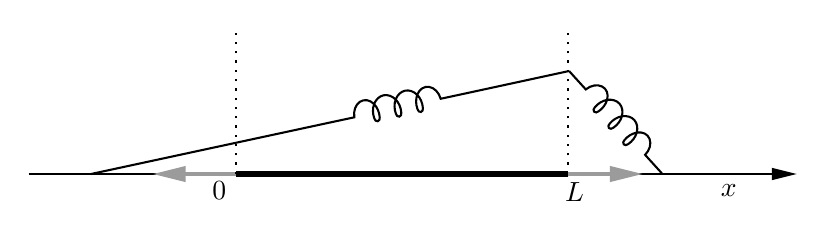
\begin{tikzpicture}[x=0.75pt,y=0.75pt,yscale=-1,xscale=1]
                  %uncomment if require: \path (0,109); %set diagram left start at 0, and has height of 109

                  %Straight Lines [id:da8183608339237425] 
                  \draw    (50,80) -- (418,80) ;
                  \draw [shift={(420,80)}, rotate = 180] [fill={rgb, 255:red, 0; green, 0; blue, 0 }  ][line width=0.08]  [draw opacity=0] (12,-3) -- (0,0) -- (12,3) -- cycle    ;
                  %Straight Lines [id:da3482453921514461] 
                  \draw  [dash pattern={on 0.84pt off 2.51pt}]  (310,80) -- (310,10) ;
                  %Straight Lines [id:da07897086281752164] 
                  \draw [color={rgb, 255:red, 155; green, 155; blue, 155 }  ,draw opacity=1 ][line width=1.5]    (310,80) -- (341.64,80) ;
                  \draw [shift={(345.64,80)}, rotate = 180] [fill={rgb, 255:red, 155; green, 155; blue, 155 }  ,fill opacity=1 ][line width=0.08]  [draw opacity=0] (15.6,-3.9) -- (0,0) -- (15.6,3.9) -- cycle    ;
                  %Straight Lines [id:da32349814463136983] 
                  \draw [color={rgb, 255:red, 155; green, 155; blue, 155 }  ,draw opacity=1 ][line width=1.5]    (150,80) -- (114,80) ;
                  \draw [shift={(110,80)}, rotate = 360] [fill={rgb, 255:red, 155; green, 155; blue, 155 }  ,fill opacity=1 ][line width=0.08]  [draw opacity=0] (15.6,-3.9) -- (0,0) -- (15.6,3.9) -- cycle    ;
                  %Shape: Inductor (Air Core) [id:dp770920514520002] 
                  \draw   (310.35,30.38) -- (318.39,39.25) .. controls (320.82,37.27) and (323.92,36.7) .. (326.19,37.82) .. controls (328.47,38.93) and (329.45,41.5) .. (328.67,44.28) .. controls (328.05,46.44) and (326.55,48.46) .. (324.55,49.82) .. controls (323.85,50.45) and (322.89,50.51) .. (322.4,49.97) .. controls (321.9,49.43) and (322.07,48.48) .. (322.76,47.85) .. controls (324.3,45.98) and (326.46,44.68) .. (328.67,44.28) .. controls (331.11,43.94) and (333.25,44.59) .. (334.6,46.08) .. controls (335.96,47.57) and (336.39,49.77) .. (335.82,52.16) .. controls (335.2,54.32) and (333.7,56.34) .. (331.69,57.7) .. controls (331,58.33) and (330.04,58.39) .. (329.54,57.85) .. controls (329.05,57.31) and (329.21,56.36) .. (329.9,55.73) .. controls (331.45,53.86) and (333.6,52.57) .. (335.82,52.16) .. controls (338.25,51.82) and (340.4,52.47) .. (341.75,53.96) .. controls (343.1,55.45) and (343.54,57.65) .. (342.96,60.04) .. controls (342.34,62.21) and (340.84,64.22) .. (338.84,65.58) .. controls (338.14,66.21) and (337.18,66.27) .. (336.69,65.73) .. controls (336.2,65.19) and (336.36,64.24) .. (337.05,63.61) .. controls (338.6,61.74) and (340.75,60.45) .. (342.96,60.04) .. controls (345.81,59.54) and (348.27,60.77) .. (349.15,63.14) .. controls (350.04,65.51) and (349.17,68.54) .. (346.97,70.77) -- (355.01,79.63) ;
                  %Shape: Inductor (Air Core) [id:dp950587555474834] 
                  \draw   (195.17,55.19) -- (206.88,52.68) .. controls (206.39,49.58) and (207.45,46.62) .. (209.55,45.21) .. controls (211.66,43.8) and (214.37,44.24) .. (216.39,46.31) .. controls (217.95,47.93) and (218.94,50.24) .. (219.11,52.65) .. controls (219.31,53.57) and (218.88,54.43) .. (218.16,54.59) .. controls (217.45,54.74) and (216.71,54.12) .. (216.51,53.21) .. controls (215.67,50.94) and (215.63,48.42) .. (216.39,46.31) .. controls (217.31,44.03) and (218.95,42.5) .. (220.92,42.08) .. controls (222.89,41.65) and (225.01,42.38) .. (226.79,44.08) .. controls (228.35,45.69) and (229.34,48.01) .. (229.51,50.42) .. controls (229.71,51.33) and (229.28,52.2) .. (228.57,52.36) .. controls (227.85,52.51) and (227.11,51.89) .. (226.91,50.98) .. controls (226.07,48.71) and (226.03,46.19) .. (226.79,44.08) .. controls (227.71,41.8) and (229.35,40.27) .. (231.32,39.85) .. controls (233.29,39.42) and (235.41,40.15) .. (237.19,41.85) .. controls (238.75,43.46) and (239.74,45.77) .. (239.91,48.19) .. controls (240.11,49.1) and (239.68,49.97) .. (238.97,50.12) .. controls (238.25,50.28) and (237.51,49.66) .. (237.31,48.75) .. controls (236.47,46.48) and (236.43,43.96) .. (237.19,41.85) .. controls (238.18,39.13) and (240.48,37.62) .. (242.97,38.04) .. controls (245.47,38.46) and (247.65,40.73) .. (248.48,43.75) -- (260.18,41.24) ;
                  %Straight Lines [id:da1546928964586438] 
                  \draw    (310.35,30.38) -- (260.18,41.24) ;
                  %Straight Lines [id:da853014356746008] 
                  \draw    (195.17,55.19) -- (80,80) ;
                  %Straight Lines [id:da7915524502268632] 
                  \draw [line width=2.25]    (310,80) -- (150,80) ;
                  %Straight Lines [id:da550897476154729] 
                  \draw  [dash pattern={on 0.84pt off 2.51pt}]  (150,80) -- (150,10) ;

                  % Text Node
                  \draw (137,82.4) node [anchor=north west][inner sep=0.75pt]    {$0$};
                  % Text Node
                  \draw (307,82.4) node [anchor=north west][inner sep=0.75pt]    {$L$};
                  % Text Node
                  \draw (382,83.4) node [anchor=north west][inner sep=0.75pt]    {$x$};

              \end{tikzpicture}
          \end{figure}
          \FloatBarrier
          Osserviamo che se $k=0$ ritroviamo le condizioni di Neumann omogenee, ciò ha senso dato che è come avere una molla che pone una resistenza nulla, ovvero la corda è libera di scorrere in verticale. Viceversa se $\displaystyle k\gg \{u,u_{x}\}$ allora $u$ per compensare deve essere molto picolo, è come avere una molla rigidissima che sostanzialmente impone di fissare gli estremi, come nella condizione di Dirichlet.\footnote{Si veda \texttt{https://youtu.be/AEBdyFG3bz4} per ulteriori chiarificazioni.}
\end{itemize}
\section{Problema di Cauchy globale \texorpdfstring{($n=1$)}{(n=1)}}

Si dice problema di Cauchy globale
\begin{equation*}
    \begin{cases}
        u_{tt} -c^{2} u_{xx} =f     & x\in \mathbb{R} ,\ t >0 \\
        \begin{array}{l}
            u(x,0) =g(x) , \\
            u_{t}(x,0) =h(x)
        \end{array} & x\in \mathbb{R}
    \end{cases}
\end{equation*}
Risolviamo il Problema di Cauchy \textit{omogeneo} ($f=0$) per arrivare alla \textbf{Formula di d'Alembert.}
\begin{equation*}
    \begin{cases}
        u_{tt} -c^{2} u_{xx} =0     & x\in \mathbb{R} ,\ t >0 \\
        \begin{array}{l}
            u(x,0) =g(x) , \\
            u_{t}(x,0) =h(x)
        \end{array} & x\in \mathbb{R}
    \end{cases}
\end{equation*}
\begin{nb}
    Come visto in Sezione \vref{sec:leggi-conservazione-non-omogeneo}, la soluzione di un'equazione del tipo
    \begin{equation*}
        u_{t} \pm cu_{x} =f(x,t) \ \ x\in \mathbb{R} ,\ t >0
    \end{equation*}
    è data da
    \begin{equation}
        u(x,t) =\varphi (x\mp ct) +\int ^{t}_{0} f(x \mp c(t-s) ,s) \ds
        \label{eq:premessa-d-alembert}
    \end{equation}
\end{nb}
Fattorizziamo l'equazione della corda e definiamo una funzione $v$
\begin{equation*}
    u_{tt} -c^{2} u_{xx} =(\partial _{t} -c\partial _{x})\underbrace{(\partial _{t} +c\partial _{x}) u}_{v} =0
\end{equation*}
allora
\begin{equation*}
    v_{t} -cv_{x} =0
\end{equation*}
ma noi la sappiamo risolvere grazie a \eqref{eq:premessa-d-alembert}
\begin{equation*}
    v(x,t) =\varphi (x+ct)
\end{equation*}
a questo punto dobbiamo semplicemente risolvere
\begin{equation*}
    \underbrace{u_{t} +cu_{x}}_{(\partial _{t} +c\partial _{x}) u} =\underbrace{\varphi (x+ct)}_{v(x,t)}
\end{equation*}
sempre grazie a \eqref{eq:premessa-d-alembert}
\begin{align*}
    u(x,t) & =\psi (x-ct) +\int ^{t}_{0} \varphi (x-c(t-s) +cs) \ds \\
           & =\psi (x-ct) +\int ^{t}_{0} \varphi (x-ct+2cs) \ds
\end{align*}
per sostituzione
\begin{equation*}
    x-ct+2cs=y\ \ \Rightarrow \ \ \begin{cases}
        \ds=\frac{1}{2c} \dy &        \\
        s=0:                 & y=x-ct \\
        s=t:                 & y=x+ct
    \end{cases}
\end{equation*}
allora
\begin{equation}
    u(x,t) =\psi (x-ct) +\frac{1}{2c}\int ^{x+ct}_{x-ct} \varphi (y) \dy
    \label{eq:d-alembert-intermedio}
\end{equation}
Il problema è ora determinare $\varphi ,\psi $ in modo che siano verificate le condizioni iniziali
\begin{equation*}
    u(x,0) =g(x) ,\ \ u_{t}(x,0) =h(x)
\end{equation*}
da cui
\begin{align*}
    u(x,0)     & =\psi (x) =g(x) \ \ \Rightarrow \ \ \boxed{\psi (x) =g(x)}                        \\
               &                                                                                   \\
    u_{t}(x,t) & =-cg'(x-ct) +\frac{1}{2c}[ \varphi (x+ct) c-\varphi (x-ct)(-c)]                   \\
               & =-cg'(x-ct) +\frac{1}{2}[ \varphi (x+ct) +\varphi (x-ct)]                         \\
    u_{t}(x,0) & =-cg'(x) +\varphi (x) =h(x) \ \ \Rightarrow \ \ \boxed{\varphi (x) =h(x) +cg'(x)}
\end{align*}
Sostituiamo nella \eqref{eq:d-alembert-intermedio}
\begin{equation*}
    u(x,t) =g(x-ct) +\frac{1}{2c}\int ^{x+ct}_{x-ct}[ h(y) +cg'(y)] \dy
\end{equation*}
Ma separando i due termini dell'integrale, per il Teorema Fondamentale del Calcolo
\begin{align*}
    u(x,t) & =g(x-ct) +\frac{1}{2c}\int ^{x+ct}_{x-ct} h(y) \dy+\frac{1}{2}\int ^{x+ct}_{x-ct} g'(y) \dy \\
           & =g(x-ct) +\frac{1}{2c}\int ^{x+ct}_{x-ct} h(y) \dy+\frac{1}{2}[ g(x+ct) -g(x-ct)]
\end{align*}
Ottengo la \textbf{formula di d'Alembert}
\begin{equation}
    \boxed{u(x,t) =\frac{1}{2}[ g(x-ct) +g(x+ct)] +\frac{1}{2c}\int ^{x+ct}_{x-ct} h(y) \dy}
\end{equation}
$u,g$ sono lunghezze, $h$ è una velocità, l'integrale è spazio$^{2}$/tempo, ma è diviso per $c$ che è spazio/tempo, quindi torna uno spazio.

Il valore di $u$ nel punto $(x,t)$ dipende dalla media dei valori di $g$ in $x\pm ct$ + la media integrale dei valori di $h$ sull'intervallo $[ x\pm ct]$, che si chiama \textbf{dominio di dipendenza}.

\begin{figure}[htpb]
    \centering
    \tikzset{every picture/.style={line width=0.75pt}} %set default line width to 0.75pt        

    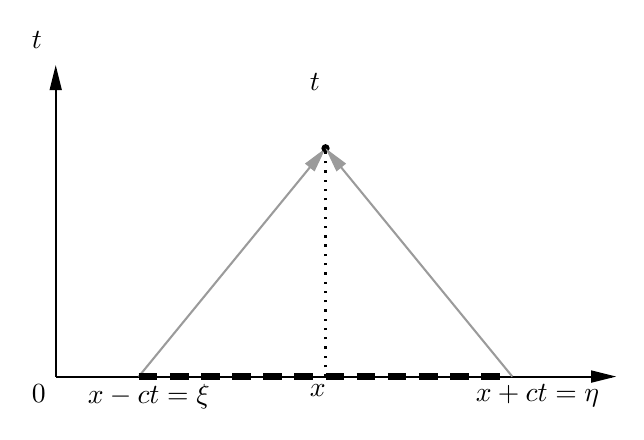
\begin{tikzpicture}[x=0.75pt,y=0.75pt,yscale=-1,xscale=1]
        %uncomment if require: \path (0,215); %set diagram left start at 0, and has height of 215

        %Straight Lines [id:da014964752359748257] 
        \draw    (170,170) -- (438,170) ;
        \draw [shift={(440,170)}, rotate = 180] [fill={rgb, 255:red, 0; green, 0; blue, 0 }  ][line width=0.08]  [draw opacity=0] (12,-3) -- (0,0) -- (12,3) -- cycle    ;
        %Straight Lines [id:da9561233996679481] 
        \draw [color={rgb, 255:red, 155; green, 155; blue, 155 }  ,draw opacity=1 ]   (210,170) -- (298.73,61.55) ;
        \draw [shift={(300,60)}, rotate = 489.29] [fill={rgb, 255:red, 155; green, 155; blue, 155 }  ,fill opacity=1 ][line width=0.08]  [draw opacity=0] (12,-3) -- (0,0) -- (12,3) -- cycle    ;
        %Straight Lines [id:da9904495944733138] 
        \draw    (170,170) -- (170,22) ;
        \draw [shift={(170,20)}, rotate = 450] [fill={rgb, 255:red, 0; green, 0; blue, 0 }  ][line width=0.08]  [draw opacity=0] (12,-3) -- (0,0) -- (12,3) -- cycle    ;
        %Shape: Ellipse [id:dp37001048028669503] 
        \draw  [draw opacity=0][fill={rgb, 255:red, 0; green, 0; blue, 0 }  ,fill opacity=1 ] (298,60) .. controls (298,58.9) and (298.9,58) .. (300,58) .. controls (301.1,58) and (302,58.9) .. (302,60) .. controls (302,61.1) and (301.1,62) .. (300,62) .. controls (298.9,62) and (298,61.1) .. (298,60) -- cycle ;
        %Straight Lines [id:da8569479996915415] 
        \draw [color={rgb, 255:red, 155; green, 155; blue, 155 }  ,draw opacity=1 ]   (390,170) -- (301.27,61.55) ;
        \draw [shift={(300,60)}, rotate = 410.71000000000004] [fill={rgb, 255:red, 155; green, 155; blue, 155 }  ,fill opacity=1 ][line width=0.08]  [draw opacity=0] (12,-3) -- (0,0) -- (12,3) -- cycle    ;
        %Straight Lines [id:da08668256662707452] 
        \draw  [dash pattern={on 0.84pt off 2.51pt}]  (300,170) -- (300,60) ;
        %Straight Lines [id:da5264911529477336] 
        \draw [line width=2.25]  [dash pattern={on 6.75pt off 4.5pt}]  (210,170) -- (390,170) ;

        % Text Node
        \draw (157,172.4) node [anchor=north west][inner sep=0.75pt]    {$0$};
        % Text Node
        \draw (291,172.4) node [anchor=north west][inner sep=0.75pt]    {$x$};
        % Text Node
        \draw (184,172.4) node [anchor=north west][inner sep=0.75pt]    {$x-ct=\xi $};
        % Text Node
        \draw (371,172.4) node [anchor=north west][inner sep=0.75pt]    {$x+ct=\eta $};
        % Text Node
        \draw (157,2.4) node [anchor=north west][inner sep=0.75pt]    {$t$};
        % Text Node
        \draw (291,22.4) node [anchor=north west][inner sep=0.75pt]    {$t$};

    \end{tikzpicture}
\end{figure}
\FloatBarrier

La formula di d'Alembert si può scrivere come sovrapposizione di onde progressive
\begin{equation*}
    u(x,t) =F(x-ct) +G(x+ct)
\end{equation*}
\begin{itemize}
    \item $F$ che viaggia verso \textit{destra} con velocità $c$
    \item $G$ che viaggia verso \textit{sinistra} con velocità $c$
\end{itemize}

$F,G$ sono costanti lungo le rette del tipo
\begin{gather*}
    F\ \Rightarrow \ \gamma ^{+} :\ x-ct=\xi \\
    G\ \Rightarrow \ \gamma ^{-} :\ x+ct=\eta
\end{gather*}
sono dette \textbf{rette caratteristiche. }Il dato iniziale viene trasportato lungo queste due rette per contribuire al valore in $(x,t)$.

Da un altro punto di vista, se facciamo partire le due caratteristiche da $z$

\begin{figure}[htpb]
    \centering
    \tikzset{every picture/.style={line width=0.75pt}} %set default line width to 0.75pt        

    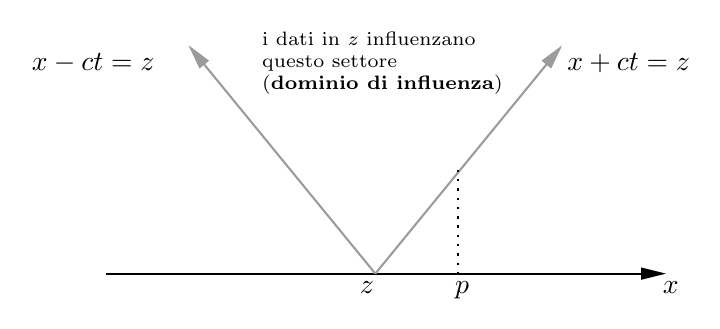
\begin{tikzpicture}[x=0.75pt,y=0.75pt,yscale=-1,xscale=1]
        %uncomment if require: \path (0,162); %set diagram left start at 0, and has height of 162

        %Straight Lines [id:da87670838095282] 
        \draw    (160,140) -- (428,140) ;
        \draw [shift={(430,140)}, rotate = 180] [fill={rgb, 255:red, 0; green, 0; blue, 0 }  ][line width=0.08]  [draw opacity=0] (12,-3) -- (0,0) -- (12,3) -- cycle    ;
        %Straight Lines [id:da25392995285217457] 
        \draw [color={rgb, 255:red, 155; green, 155; blue, 155 }  ,draw opacity=1 ]   (290,140) -- (378.73,31.55) ;
        \draw [shift={(380,30)}, rotate = 489.29] [fill={rgb, 255:red, 155; green, 155; blue, 155 }  ,fill opacity=1 ][line width=0.08]  [draw opacity=0] (12,-3) -- (0,0) -- (12,3) -- cycle    ;
        %Straight Lines [id:da9039716060651264] 
        \draw [color={rgb, 255:red, 155; green, 155; blue, 155 }  ,draw opacity=1 ]   (290,140) -- (201.27,31.55) ;
        \draw [shift={(200,30)}, rotate = 410.71000000000004] [fill={rgb, 255:red, 155; green, 155; blue, 155 }  ,fill opacity=1 ][line width=0.08]  [draw opacity=0] (12,-3) -- (0,0) -- (12,3) -- cycle    ;
        %Straight Lines [id:da06694332321834096] 
        \draw  [dash pattern={on 0.84pt off 2.51pt}]  (330,90) -- (330,140) ;

        % Text Node
        \draw (281,142.4) node [anchor=north west][inner sep=0.75pt]    {$z$};
        % Text Node
        \draw (123,32.4) node [anchor=north west][inner sep=0.75pt]    {$x-ct=z$};
        % Text Node
        \draw (381,32.4) node [anchor=north west][inner sep=0.75pt]    {$x+ct=z$};
        % Text Node
        \draw (234,22) node [anchor=north west][inner sep=0.75pt]  [font=\scriptsize] [align=left] {i dati in $z$ influenzano\\questo settore\\(\textbf{dominio di influenza})};
        % Text Node
        \draw (427,142.4) node [anchor=north west][inner sep=0.75pt]    {$x$};
        % Text Node
        \draw (327,142.4) node [anchor=north west][inner sep=0.75pt]    {$p$};

    \end{tikzpicture}
\end{figure}
\FloatBarrier
Una perturbazione inizialmente localizzata in $z$ non viene avvertita nel punto $p$ fino al tempo
\begin{equation*}
    \overline{t} =\frac{| p-z| }{c}
\end{equation*}
e poi viene continuata ad essere avvertita anche per tempi successivi perché rimane nel settore.

Nel caso invece in cui il dato è trasportato esclusivamente lungo la caratteristica il segnale è istantaneo, tale caso si ha quando $h=0$.

Questo evidenzia la caratteristica intermedia del caso in dimensione $n=1$, mentre vedremo che la caratteristica di ammettere segnali istantanei dipende dalla dimensione $n$ dello spazio, se è pari o dispari.

\LezioneS{08/04/2021}

Riprendiamo il \textbf{problema di Cauchy globale} omogeneo.
\begin{equation}
    \tag{PCG$_{\text{onde,1D}}$} \
    \begin{cases}
        u_{tt} -c^{2} u_{xx} =0 & x\in \mathbb{R} ,t >0 \\
        u(x,0) =g(x)            & x\in \mathbb{R}       \\
        u_{t}(x,0) =h(x)        & x\in \mathbb{R}
    \end{cases}
    \label{eq:pcg-onde-1d}
\end{equation}
la soluzione è data dalla \textbf{formula di d'Alembert}
\begin{equation}
    u(x,t) =\frac{1}{2}[ g(x+ct) +g(x-ct)] +\frac{1}{2c}\int _{x-ct}^{x+ct} h(y) \dy
    \label{eq:onde-formula-di-dAlembert}
\end{equation}
Esaminiamo alcune conseguenze di questa formula:
\begin{enumerate}
    \item Il \eqref{eq:pcg-onde-1d} ha un'\textbf{unica} soluzione \textit{regolare} data da \eqref{eq:onde-formula-di-dAlembert}. Notiamo che deve essere:
          \begin{equation*}
              g\in C^{2}(\mathbb{R}) ,\ h\in C^{1}(\mathbb{R}) ,
          \end{equation*}
          affinché $u$ sia\textbf{ soluzione classica}. Non c'è regolarizzazione all'avanzare del tempo.
    \item Posso ricavare una stima di stabilità in norma $\displaystyle L^{\infty }$ con la formula di d'Alembert. Consideriamo
          \begin{equation*}
              g_{1} ,g_{2} ,\ h_{1} ,h_{2}\rightarrow u_{1} ,u_{2}
          \end{equation*}
          allora
          \begin{equation*}
              | u_{1}(x,t) -u_{2}(x,t)| \leq \Vert g_{1} -g_{2}\Vert _{L^{\infty }(\mathbb{R})} +T\Vert h_{1} -h_{2}\Vert _{L^{\infty }(\mathbb{R})}
          \end{equation*}
          per ogni $x\in \mathbb{R}, t\in [0,T]$.
    \item La $u$ si può esprimere come somma di due funzioni
          \begin{equation*}
              u(x,t) =F(x-ct) +G(x+ct)
          \end{equation*}
          per esempio
          \begin{align*}
              F(x+ct) & =\frac{1}{2} g(x+ct) +\frac{1}{2c}\int _{0}^{x+ct} h(y) \dy \\
              G(x-ct) & =\frac{1}{2} g(x-ct) +\frac{1}{2c}\int _{x-ct}^{0} h(y) \dy
          \end{align*}
          quindi $u$ è sovrapposizione di due onde progressive.
    \item Nonostante abbiamo assunto $\displaystyle g\in C^{2} ,\ h\in C^{1}$ la Formula di d'Alembert \eqref{eq:onde-formula-di-dAlembert} ha senso anche per $g$ continua e $h$ limitata e soddisfa l'equazione in un senso \textit{debole}
          \fg[Corda pizzicata in un punto]{0.6}{onde-corda-pizzicata-in-un-punto}

    \item Domini di \textbf{dipendenza} e di \textbf{influenza:}
          \fg[Domini di dipendenza e di influenza]{0.6}{onde-domini-dipendenza-influenza}


          $g$ influisce sul valore $\displaystyle u(x,t)$ solo dai punti $\displaystyle (x-ct,0) ,(x+ct,0)$.

          I valori di $h$ che influiscono su $\displaystyle u(x,t)$ sono quelli dell'intero intervallo $\displaystyle [ x-ct,x+ct]$, detto \textbf{dominio di dipendenza }del punto $\displaystyle (x,t)$.
    \item \textbf{Quadrilatero caratteristico}. Le rette:
          \begin{align*}
              x-ct & =\xi \\
              x+ct & =\mu
          \end{align*}
          sono le rette caratteristiche \emph{che trasportano i dati iniziali}
          \begin{figure}[htpb]
              \centering

              \tikzset{every picture/.style={line width=0.75pt}} %set default line width to 0.75pt        

              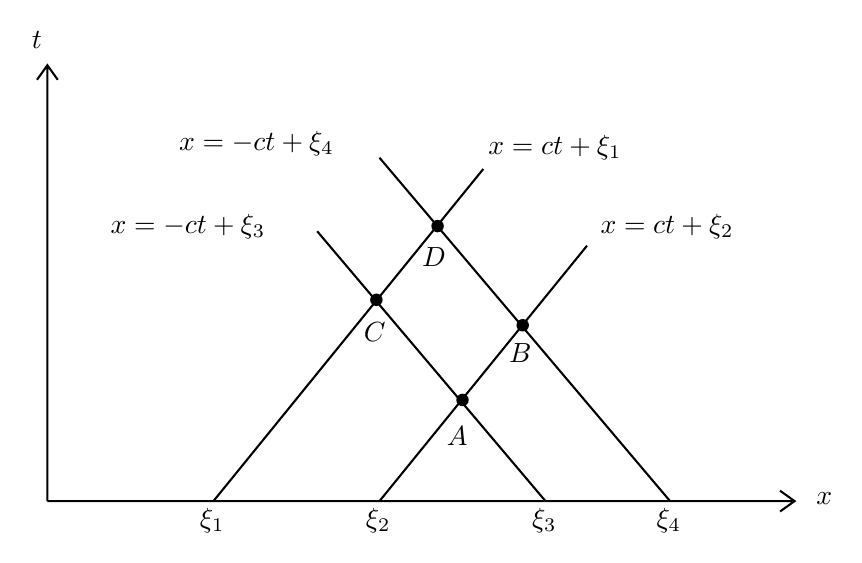
\begin{tikzpicture}[x=0.75pt,y=0.75pt,yscale=-1,xscale=1]
                  %uncomment if require: \path (0,300); %set diagram left start at 0, and has height of 300

                  %Shape: Axis 2D [id:dp5446048811905655] 
                  \draw  (90,260) -- (450,260)(90,50) -- (90,260) -- cycle (443,255) -- (450,260) -- (443,265) (85,57) -- (90,50) -- (95,57)  ;
                  %Straight Lines [id:da957953326055226] 
                  \draw    (350,136.92) -- (250,260) ;
                  %Straight Lines [id:da929763421955655] 
                  \draw    (300,100) -- (170,260) ;
                  %Straight Lines [id:da7318835798607295] 
                  \draw    (220,130) -- (330,260) ;
                  %Straight Lines [id:da5952857018004307] 
                  \draw    (250,94.55) -- (390,260) ;
                  %Shape: Circle [id:dp5681242877578812] 
                  \draw  [draw opacity=0][fill={rgb, 255:red, 0; green, 0; blue, 0 }  ,fill opacity=1 ] (245.5,163) .. controls (245.5,161.34) and (246.84,160) .. (248.5,160) .. controls (250.16,160) and (251.5,161.34) .. (251.5,163) .. controls (251.5,164.66) and (250.16,166) .. (248.5,166) .. controls (246.84,166) and (245.5,164.66) .. (245.5,163) -- cycle ;
                  %Shape: Circle [id:dp7348122693316455] 
                  \draw  [draw opacity=0][fill={rgb, 255:red, 0; green, 0; blue, 0 }  ,fill opacity=1 ] (275,127.5) .. controls (275,125.84) and (276.34,124.5) .. (278,124.5) .. controls (279.66,124.5) and (281,125.84) .. (281,127.5) .. controls (281,129.16) and (279.66,130.5) .. (278,130.5) .. controls (276.34,130.5) and (275,129.16) .. (275,127.5) -- cycle ;
                  %Shape: Circle [id:dp06799940585538478] 
                  \draw  [draw opacity=0][fill={rgb, 255:red, 0; green, 0; blue, 0 }  ,fill opacity=1 ] (316,175.27) .. controls (316,173.62) and (317.34,172.27) .. (319,172.27) .. controls (320.66,172.27) and (322,173.62) .. (322,175.27) .. controls (322,176.93) and (320.66,178.27) .. (319,178.27) .. controls (317.34,178.27) and (316,176.93) .. (316,175.27) -- cycle ;
                  %Shape: Circle [id:dp44710284173444226] 
                  \draw  [draw opacity=0][fill={rgb, 255:red, 0; green, 0; blue, 0 }  ,fill opacity=1 ] (287,211.27) .. controls (287,209.62) and (288.34,208.27) .. (290,208.27) .. controls (291.66,208.27) and (293,209.62) .. (293,211.27) .. controls (293,212.93) and (291.66,214.27) .. (290,214.27) .. controls (288.34,214.27) and (287,212.93) .. (287,211.27) -- cycle ;

                  % Text Node
                  \draw (459,254.4) node [anchor=north west][inner sep=0.75pt]    {$x$};
                  % Text Node
                  \draw (81,32.4) node [anchor=north west][inner sep=0.75pt]    {$t$};
                  % Text Node
                  \draw (281,222.4) node [anchor=north west][inner sep=0.75pt]    {$A$};
                  % Text Node
                  \draw (311,182.4) node [anchor=north west][inner sep=0.75pt]    {$B$};
                  % Text Node
                  \draw (241,172.4) node [anchor=north west][inner sep=0.75pt]    {$C$};
                  % Text Node
                  \draw (269,136.4) node [anchor=north west][inner sep=0.75pt]    {$D$};
                  % Text Node
                  \draw (162,261.9) node [anchor=north west][inner sep=0.75pt]    {$\xi _{1}$};
                  % Text Node
                  \draw (242,261.9) node [anchor=north west][inner sep=0.75pt]    {$\xi _{2}$};
                  % Text Node
                  \draw (322,261.9) node [anchor=north west][inner sep=0.75pt]    {$\xi _{3}$};
                  % Text Node
                  \draw (382,261.9) node [anchor=north west][inner sep=0.75pt]    {$\xi _{4}$};
                  % Text Node
                  \draw (301,82.4) node [anchor=north west][inner sep=0.75pt]    {$x=ct+\xi _{1}$};
                  % Text Node
                  \draw (355,120.4) node [anchor=north west][inner sep=0.75pt]    {$x=ct+\xi _{2}$};
                  % Text Node
                  \draw (152,80.4) node [anchor=north west][inner sep=0.75pt]    {$x=-ct+\xi _{4}$};
                  % Text Node
                  \draw (119,120.4) node [anchor=north west][inner sep=0.75pt]    {$x=-ct+\xi _{3}$};

              \end{tikzpicture}
          \end{figure}
          \FloatBarrier

          ricordando che
          \begin{equation*}
              u(x,t) =F(x-ct) +G(x+ct)
          \end{equation*}

          deduciamo che sulle rette $\displaystyle x=-ct+\xi $, $G$ è costante, sulle rette $\displaystyle x=ct+\xi $, $F$ è costante. Ma allora:
          \begin{align*}
              F(A) & =F(B) \\
              G(A) & =G(C) \\
              F(D) & =F(C) \\
              G(D) & =G(B)
          \end{align*}

          sommo membro a membro e ottengo
          \begin{equation*}
              \underbrace{F(A) +G(A)}_{u(A)} +\underbrace{F(D) +G(D)}_{u(D)} =\underbrace{F(B) +G(B)}_{u(B)} +\underbrace{F(C) +G(C)}_{u(C)}
          \end{equation*}

          cioè:

          \begin{equation}
              u(A) +u(D) -u(B) -u(C) =0.
              \label{eq:onde-uguaglianze-quadrilatero}
          \end{equation}

          Se è verificata per ogni coppia di caratteristiche questa esprime l'equazione delle onde \textbf{in forma debole.}

          Usiamo la \eqref{eq:onde-uguaglianze-quadrilatero} per risolvere il problema di Cauchy-Dirichlet
          \begin{equation*}
              \begin{cases}
                  u_{tt} -u_{xx} =0 & 0< x< L,\ t >0          \\
                  u(x,0) =g(x)      & 0\leq x\leq L \\
                  u_{t}(x,0) =h(x)  & 0\leq x\leq L \\
                  u(0,t) =a(t)      & t >0                    \\
                  u(L,t) =b(t)      & t >0
              \end{cases}
          \end{equation*}

          con un'argomentazione puramente \textit{visuale}:

          \begin{figure}[htpb]
              \centering
              \tikzset{every picture/.style={line width=0.75pt}} %set default line width to 0.75pt        

              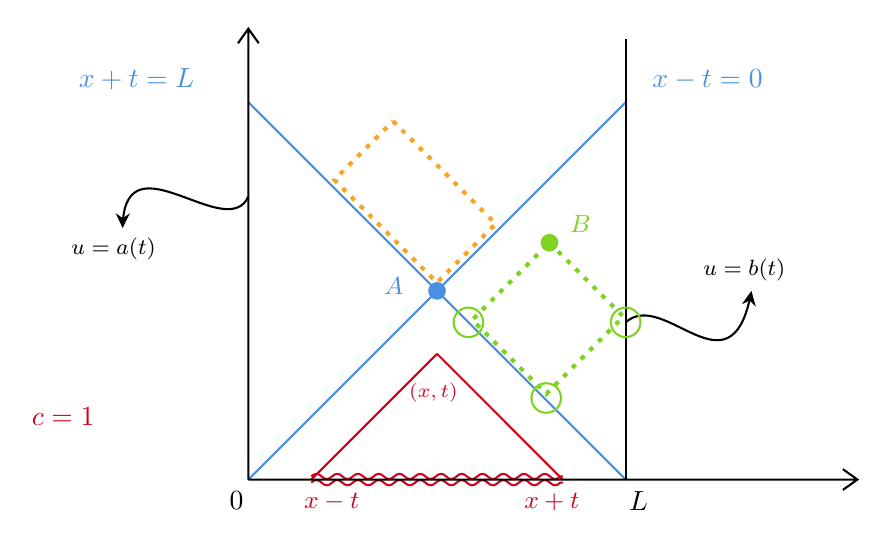
\begin{tikzpicture}[x=0.75pt,y=0.75pt,yscale=-1,xscale=1]
                  %uncomment if require: \path (0,287); %set diagram left start at 0, and has height of 287

                  %Straight Lines [id:da585347869552219] 
                  \draw [color={rgb, 255:red, 74; green, 144; blue, 226 }  ,draw opacity=1 ]   (167.57,65.44) -- (349.34,247.21) ;
                  %Straight Lines [id:da824218001234857] 
                  \draw [color={rgb, 255:red, 74; green, 144; blue, 226 }  ,draw opacity=1 ]   (349.34,65.44) -- (167.57,247.21) ;
                  %Straight Lines [id:da17362039318852585] 
                  \draw [color={rgb, 255:red, 208; green, 2; blue, 27 }  ,draw opacity=1 ]   (258.46,186.62) -- (319.04,247.21) ;
                  %Straight Lines [id:da16420672299248373] 
                  \draw [color={rgb, 255:red, 208; green, 2; blue, 27 }  ,draw opacity=1 ]   (258.46,186.62) -- (197.87,247.21) ;
                  %Straight Lines [id:da49220817930888017] 
                  \draw [color={rgb, 255:red, 208; green, 2; blue, 27 }  ,draw opacity=1 ]   (197.87,245.71) .. controls (199.54,244.04) and (201.2,244.04) .. (202.87,245.71) .. controls (204.54,247.38) and (206.2,247.38) .. (207.87,245.71) .. controls (209.54,244.04) and (211.2,244.04) .. (212.87,245.71) .. controls (214.54,247.38) and (216.2,247.38) .. (217.87,245.71) .. controls (219.54,244.04) and (221.2,244.04) .. (222.87,245.71) .. controls (224.54,247.38) and (226.2,247.38) .. (227.87,245.71) .. controls (229.54,244.04) and (231.2,244.04) .. (232.87,245.71) .. controls (234.54,247.38) and (236.2,247.38) .. (237.87,245.71) .. controls (239.54,244.04) and (241.2,244.04) .. (242.87,245.71) .. controls (244.54,247.38) and (246.2,247.38) .. (247.87,245.71) .. controls (249.54,244.04) and (251.2,244.04) .. (252.87,245.71) .. controls (254.54,247.38) and (256.2,247.38) .. (257.87,245.71) .. controls (259.54,244.04) and (261.2,244.04) .. (262.87,245.71) .. controls (264.54,247.38) and (266.2,247.38) .. (267.87,245.71) .. controls (269.54,244.04) and (271.2,244.04) .. (272.87,245.71) .. controls (274.54,247.38) and (276.2,247.38) .. (277.87,245.71) .. controls (279.54,244.04) and (281.2,244.04) .. (282.87,245.71) .. controls (284.54,247.38) and (286.2,247.38) .. (287.87,245.71) .. controls (289.54,244.04) and (291.2,244.04) .. (292.87,245.71) .. controls (294.54,247.38) and (296.2,247.38) .. (297.87,245.71) .. controls (299.54,244.04) and (301.2,244.04) .. (302.87,245.71) .. controls (304.54,247.38) and (306.2,247.38) .. (307.87,245.71) .. controls (309.54,244.04) and (311.2,244.04) .. (312.87,245.71) .. controls (314.54,247.38) and (316.2,247.38) .. (317.87,245.71) -- (319.04,245.71) -- (319.04,245.71)(197.87,248.71) .. controls (199.54,247.04) and (201.2,247.04) .. (202.87,248.71) .. controls (204.54,250.38) and (206.2,250.38) .. (207.87,248.71) .. controls (209.54,247.04) and (211.2,247.04) .. (212.87,248.71) .. controls (214.54,250.38) and (216.2,250.38) .. (217.87,248.71) .. controls (219.54,247.04) and (221.2,247.04) .. (222.87,248.71) .. controls (224.54,250.38) and (226.2,250.38) .. (227.87,248.71) .. controls (229.54,247.04) and (231.2,247.04) .. (232.87,248.71) .. controls (234.54,250.38) and (236.2,250.38) .. (237.87,248.71) .. controls (239.54,247.04) and (241.2,247.04) .. (242.87,248.71) .. controls (244.54,250.38) and (246.2,250.38) .. (247.87,248.71) .. controls (249.54,247.04) and (251.2,247.04) .. (252.87,248.71) .. controls (254.54,250.38) and (256.2,250.38) .. (257.87,248.71) .. controls (259.54,247.04) and (261.2,247.04) .. (262.87,248.71) .. controls (264.54,250.38) and (266.2,250.38) .. (267.87,248.71) .. controls (269.54,247.04) and (271.2,247.04) .. (272.87,248.71) .. controls (274.54,250.38) and (276.2,250.38) .. (277.87,248.71) .. controls (279.54,247.04) and (281.2,247.04) .. (282.87,248.71) .. controls (284.54,250.38) and (286.2,250.38) .. (287.87,248.71) .. controls (289.54,247.04) and (291.2,247.04) .. (292.87,248.71) .. controls (294.54,250.38) and (296.2,250.38) .. (297.87,248.71) .. controls (299.54,247.04) and (301.2,247.04) .. (302.87,248.71) .. controls (304.54,250.38) and (306.2,250.38) .. (307.87,248.71) .. controls (309.54,247.04) and (311.2,247.04) .. (312.87,248.71) .. controls (314.54,250.38) and (316.2,250.38) .. (317.87,248.71) -- (319.04,248.71) -- (319.04,248.71) ;
                  %Shape: Circle [id:dp9089802190336387] 
                  \draw  [draw opacity=0][fill={rgb, 255:red, 74; green, 144; blue, 226 }  ,fill opacity=1 ] (254.21,156.32) .. controls (254.21,153.98) and (256.11,152.08) .. (258.46,152.08) .. controls (260.8,152.08) and (262.7,153.98) .. (262.7,156.32) .. controls (262.7,158.67) and (260.8,160.56) .. (258.46,160.56) .. controls (256.11,160.56) and (254.21,158.67) .. (254.21,156.32) -- cycle ;
                  %Straight Lines [id:da24936660071672434] 
                  \draw    (349.34,35.15) -- (349.34,247.21) ;
                  %Curve Lines [id:da8058318016956436] 
                  \draw    (349.34,171.47) .. controls (367.72,155) and (399.53,207.63) .. (409.49,158.63) ;
                  \draw [shift={(409.93,156.32)}, rotate = 460.1] [fill={rgb, 255:red, 0; green, 0; blue, 0 }  ][line width=0.08]  [draw opacity=0] (7.14,-3.43) -- (0,0) -- (7.14,3.43) -- (4.74,0) -- cycle    ;
                  %Curve Lines [id:da49003643399916896] 
                  \draw    (167.57,110.88) .. controls (157.18,133.48) and (109.45,82.53) .. (107.07,123.41) ;
                  \draw [shift={(106.99,126.03)}, rotate = 270.63] [fill={rgb, 255:red, 0; green, 0; blue, 0 }  ][line width=0.08]  [draw opacity=0] (7.14,-3.43) -- (0,0) -- (7.14,3.43) -- (4.74,0) -- cycle    ;
                  %Shape: Circle [id:dp3785036171458238] 
                  \draw  [draw opacity=0][fill={rgb, 255:red, 126; green, 211; blue, 33 }  ,fill opacity=1 ] (308.41,133.09) .. controls (308.41,130.75) and (310.31,128.85) .. (312.65,128.85) .. controls (314.99,128.85) and (316.89,130.75) .. (316.89,133.09) .. controls (316.89,135.43) and (314.99,137.33) .. (312.65,137.33) .. controls (310.31,137.33) and (308.41,135.43) .. (308.41,133.09) -- cycle ;
                  %Shape: Ellipse [id:dp907927094458276] 
                  \draw  [color={rgb, 255:red, 126; green, 211; blue, 33 }  ,draw opacity=1 ] (266.48,171.47) .. controls (266.48,167.54) and (269.67,164.35) .. (273.6,164.35) .. controls (277.53,164.35) and (280.72,167.54) .. (280.72,171.47) .. controls (280.72,175.4) and (277.53,178.59) .. (273.6,178.59) .. controls (269.67,178.59) and (266.48,175.4) .. (266.48,171.47) -- cycle ;
                  %Shape: Ellipse [id:dp1490934708323064] 
                  \draw  [color={rgb, 255:red, 126; green, 211; blue, 33 }  ,draw opacity=1 ] (303.95,207.92) .. controls (303.95,203.99) and (307.13,200.81) .. (311.07,200.81) .. controls (315,200.81) and (318.19,203.99) .. (318.19,207.92) .. controls (318.19,211.86) and (315,215.04) .. (311.07,215.04) .. controls (307.13,215.04) and (303.95,211.86) .. (303.95,207.92) -- cycle ;
                  %Shape: Ellipse [id:dp17002319067581517] 
                  \draw  [color={rgb, 255:red, 126; green, 211; blue, 33 }  ,draw opacity=1 ] (342.22,171.47) .. controls (342.22,167.54) and (345.41,164.35) .. (349.34,164.35) .. controls (353.27,164.35) and (356.46,167.54) .. (356.46,171.47) .. controls (356.46,175.4) and (353.27,178.59) .. (349.34,178.59) .. controls (345.41,178.59) and (342.22,175.4) .. (342.22,171.47) -- cycle ;
                  %Shape: Axis 2D [id:dp7964277435601204] 
                  \draw  (167.57,247.21) -- (461,247.21)(167.57,30) -- (167.57,247.21) -- cycle (454,242.21) -- (461,247.21) -- (454,252.21) (162.57,37) -- (167.57,30) -- (172.57,37)  ;
                  %Shape: Rectangle [id:dp047903719911538856] 
                  \draw  [color={rgb, 255:red, 245; green, 166; blue, 35 }  ,draw opacity=1 ][dash pattern={on 1.69pt off 2.76pt}][line width=1.5]  (237.27,74.53) -- (286.75,124.05) -- (258.46,152.32) -- (208.98,102.81) -- cycle ;
                  %Shape: Rectangle [id:dp2346028587722877] 
                  \draw  [color={rgb, 255:red, 126; green, 211; blue, 33 }  ,draw opacity=1 ][dash pattern={on 1.69pt off 2.76pt}][line width=1.5]  (312.65,133.09) -- (348.28,168.74) -- (311.07,205.92) -- (275.44,170.27) -- cycle ;

                  % Text Node
                  \draw (157.03,251.5) node [anchor=north west][inner sep=0.75pt]    {$0$};
                  % Text Node
                  \draw (349.54,251.5) node [anchor=north west][inner sep=0.75pt]    {$L$};
                  % Text Node
                  \draw (360.71,48.19) node [anchor=north west][inner sep=0.75pt]  [color={rgb, 255:red, 74; green, 144; blue, 226 }  ,opacity=1 ]  {$x-t=0$};
                  % Text Node
                  \draw (84.43,47.69) node [anchor=north west][inner sep=0.75pt]  [color={rgb, 255:red, 74; green, 144; blue, 226 }  ,opacity=1 ]  {$x+t=L$};
                  % Text Node
                  \draw (61.74,210.97) node [anchor=north west][inner sep=0.75pt]  [font=\normalsize,color={rgb, 255:red, 208; green, 2; blue, 27 }  ,opacity=1 ]  {$c=1$};
                  % Text Node
                  \draw (243.55,199.07) node [anchor=north west][inner sep=0.75pt]  [font=\scriptsize,color={rgb, 255:red, 208; green, 2; blue, 27 }  ,opacity=1 ]  {$(x,t)$};
                  % Text Node
                  \draw (299.01,252.5) node [anchor=north west][inner sep=0.75pt]  [font=\small,color={rgb, 255:red, 208; green, 2; blue, 27 }  ,opacity=1 ]  {$x+t$};
                  % Text Node
                  \draw (192.99,252.5) node [anchor=north west][inner sep=0.75pt]  [font=\small,color={rgb, 255:red, 208; green, 2; blue, 27 }  ,opacity=1 ]  {$x-t$};
                  % Text Node
                  \draw (231.49,148.37) node [anchor=north west][inner sep=0.75pt]  [font=\small,color={rgb, 255:red, 74; green, 144; blue, 226 }  ,opacity=1 ]  {$A$};
                  % Text Node
                  \draw (385.35,139.55) node [anchor=north west][inner sep=0.75pt]  [font=\footnotesize]  {$u=b(t)$};
                  % Text Node
                  \draw (80.83,129.05) node [anchor=north west][inner sep=0.75pt]  [font=\footnotesize]  {$u=a(t)$};
                  % Text Node
                  \draw (321.13,118.54) node [anchor=north west][inner sep=0.75pt]  [font=\small,color={rgb, 255:red, 126; green, 211; blue, 33 }  ,opacity=1 ]  {$B$};


              \end{tikzpicture}
          \end{figure}
          \FloatBarrier

          nel triangolo $\displaystyle (0,L,A) \ u$ è determinata dalla Formula di d'Alembert. Nel triangolo di destra costruisco il quadrilatero caratteristico verde: conosco il valore di $u$ nei punti cerchiati in verde e \eqref{eq:onde-uguaglianze-quadrilatero} mi permette di trovare anche il valore di $\displaystyle u(B)$. Posso fare lo stesso ragionamento per ogni punto del triangolo di destra e di sinistra. Per il triangolo sopra il procedimento è analogo, costruendo un quadrilatero come quello arancione.
\end{enumerate}

\subsection{Metodo di Duhamel per il problema non omogeneo con IC omogenee.}
\begin{equation}
    \begin{cases}
        u_{tt} -c^{2} u_{xx} =f & x\in \mathbb{R} ,t >0 \\
        u(x,0) =0               & x\in \mathbb{R}       \\
        u_{t}(x,0) =0           & x\in \mathbb{R}
    \end{cases}
\end{equation}
\begin{oss}
    Ripassiamo il metodo di variazione delle costanti per il problema:
    \begin{equation*}
        \begin{cases}
            y'(t) +ay(t) =f(t) & t >0 \\
            y(0) =0            &
        \end{cases} .
    \end{equation*}
    La formula risolutiva è data da:
    \begin{equation*}
        y(t) =\int _{0}^{t}\underbrace{e^{-a(t-s)} f(s)}_{w(t;s)} \ds,
    \end{equation*}
    esaminiamo l'integranda, trattando $s$ come parametro $\displaystyle (0\leq s\leq t)$:
    \begin{equation}
        w(t;s) =e^{-a(t-s)} f(s) .
        \label{eq:osservazione-duhamel}
    \end{equation}
    $w$ soddisfa il problema di Cauchy \textit{omogeneo} con dato iniziale il secondo membro dell'equazione \eqref{eq:osservazione-duhamel} calcolato in $t=s$ (e non $t=0$):
    \begin{equation*}
        \begin{cases}
            w_{t} +aw=0  & t >s \\
            w(s,s) =f(s) & t=s
        \end{cases}
    \end{equation*}
    allora possiamo risolvere prima il problema in $w$ e poi calcolare la soluzione
    \begin{equation*}
        y(t) =\int _{0}^{t} w(t;s) \ds.
    \end{equation*}
\end{oss}

\begin{theorem}
    [Metodo di Duhamel] Se $\displaystyle w(x,t;s)$, con $\displaystyle 0\leq s\leq t$, è soluzione di
    \begin{equation*}
        \begin{cases}
            w_{tt} -c^{2} w_{xx} =\boxed{0} & x\in \mathbb{R} ,\boxed{t >s} \\
            w(x,s;s) =0                     & x\in \mathbb{R} ,t=s          \\
            w_{t}(x,s;s) =f(x,s)            & x\in \mathbb{R} ,t=s
        \end{cases}
    \end{equation*}
    allora
    \begin{equation*}
        u(x,t) =\int _{0}^{t} w(x,t;s) \ds\ \ \ \ x\in \mathbb{R} ,t >0
    \end{equation*}
    è soluzione di
    \begin{equation*}
        \begin{cases}
            u_{tt} -c^{2} u_{xx} =f & x\in \mathbb{R} ,t >0 \\
            u(x,0) =0               & x\in \mathbb{R}       \\
            u_{t}(x,0) =0           & x\in \mathbb{R}
        \end{cases}
    \end{equation*}
\end{theorem}
\begin{dimostrazione}
    Calcoliamo i vari termini
    \begin{align*}
        u_{t}(x,t)        & =\underbrace{w(x,t;t)}_{=0} +\int _{0}^{t} w_{t}(x,t;s) \ds           \\
                          &                                                                       \\
        u_{tt}(x,t)       & =\underbrace{w_{t}(x,t;t)}_{=f(x,t)} +\int _{0}^{t} w_{tt}(x,t;s) \ds \\
                          &                                                                       \\
        c^{2} u_{xx}(x,t) & =\int _{0}^{t}\underbrace{c^{2} w_{xx}(x,t;s)}_{w_{tt}(x,t;s)} \ds
    \end{align*}
    Quindi l'equazione non omogenea è rispettata
    \begin{equation*}
        u_{tt}(x,t) -c^{2} u_{xx}(x,t) =f(x,t) +\int _{0}^{t} w_{tt}(x,t;s) \ds-\int _{0}^{t} w_{tt}(x,t;s) \ds=f(x,t)
    \end{equation*}
    e anche le condizioni al bordo
    \begin{align*}
        u(x,0)     & =\int _{0}^{0} w(x,t;s) \ds=0     \\
        u_{t}(x,0) & =\int _{0}^{0} w_{t}(x,t;s) \ds=0
    \end{align*}
\end{dimostrazione}
Ottimo, ma noi tale problema lo sappiamo risolvere lo sappiamo risolvere quando $s=0$. Tuttavia l'equazione delle onde \textbf{è invariante per traslazioni temporali}, quindi usiamo la formula di d'Alembert (partendo da $s$ e non da $0$):
\begin{equation*}
    w(x,t;s) =\frac{1}{2c}\int _{x-c(t-s)}^{x+c(t-s)} f(y,s) \dy
\end{equation*}
allora grazie a Duhamel
\begin{align*}
    u(x,t) & =\int _{0}^{t} w(x,t;s) \ds                                         \\
           & =\frac{1}{2c}\int _{0}^{t}\int _{x-c(t-s)}^{x+c(t-s)} f(y,s) \dy\ds \\
           & =\frac{1}{2c}\int _{S_{x,t}} f(y,s) \dy\ds
\end{align*}
dove ricordiamo che $\displaystyle S_{x,t}$ è il settore.

\LezioneS{12/04/2021}
% (fatta da Verzini)
\section{Equazione delle onde in più dimensioni, \texorpdfstring{$n\geq 2$}{n>2}}

Affrontiamo l'equazione delle onde in più dimensioni. Studieremo l'evoluzione di $u=u(\x ,t)$. L'equazione delle onde prende la forma:
\begin{equation}
    u_{tt} -c^{2} \Delta u=f,\ \ \x \in \Omega \subset \mathbb{R}^{n} ,t >0,
\end{equation}
$c$ ha le dimensioni di una velocità anche in questo caso, e sarà la velocità di propagazione del segnale. Vi sono \textbf{particolari soluzioni}, specialmente nei casi $n=2,3$. Analizziamo il caso delle \textbf{onde sferiche} in $n=3$ e studiamo il \textbf{caso omogeneo}. La soluzione prende la forma, dipendente \textit{solo} dal raggio:
\begin{equation*}
    u(\x ,t) =w(r,t) ,\ \ r=| \x| =\sqrt{x_{1}^{2} +x_{2}^{2} +x_{3}^{2}} .
\end{equation*}
Lavoriamo in coordinate sferiche:
\begin{equation*}
    \x =
    \begin{pmatrix}
        x_{1} \\
        x_{2} \\
        x_{3}
    \end{pmatrix} =
    \begin{pmatrix}
        r\cos \vartheta \sin \psi \\
        r\sin \vartheta \sin \psi \\
        \cos \psi
    \end{pmatrix} .
\end{equation*}
\begin{nb}
    Consideriamo le coordinate sferiche in $n$ dimensioni generiche e una funzione:
    \begin{equation*}
        w=w(r,\bm{\vartheta }) ,\ \ \bm{\vartheta } \in \partial B_{1} =\mathbb{S}^{n-1} ,
    \end{equation*}
    trascuriamo la dipendenza dal tempo. $\bm{\vartheta }$ è un vettore di angoli e $\mathbb{S}^{n-1}$ indica la sfera $(n-1)$-dimensionale di raggio unitario. Il laplaciano in coordinate sferiche generiche risulta:
    \begin{equation}
        \Delta w=w_{rr} +\frac{n-1}{r} w_{r} +\frac{1}{r^{2}} \Delta _{\mathbb{S}^{n-1}} w,
    \end{equation}
    il termine $\Delta _{\mathbb{S}^{n-1}}$ è detto \textit{operatore di Laplace-Beltrami}, ed è un mostro. Nel caso particolare di $n=3$ tale operatore prende la forma:
    \begin{equation}
        \Delta _{\mathbb{S}^{n-1}} =\Delta _{\mathbb{S}^{2}} =\frac{1}{(\sin \psi)^{2}}\frac{\partial ^{2}}{\partial \vartheta ^{2}} +\frac{\partial ^{2}}{\partial \psi ^{2}} +\frac{\cos \psi }{\sin \psi }\frac{\partial }{\partial \psi } .
    \end{equation}
\end{nb}
La cosa positiva è che stiamo studiando un tipo particolare di onde, quelle sferiche, dove $w$ dipende solo dal raggio e dal tempo, non dagli angoli, per cui tutti quei termini si annullano.

L'equazione omogenea prende quindi la forma:
\begin{equation}
    w_{tt} -c^{2}\left(w_{rr} +\frac{\textcolor[rgb]{0.82,0.01,0.11}{2}}{r} w_{r} +0\right) =0.
    \label{eq:equazione-onde-omogenea-polare-n-3}
\end{equation}
Quello che stiamo per fare funziona solo in dimensione $3$ perché nella parentesi c'è il $\textcolor[rgb]{0.82,0.01,0.11}{2}$, che viene da $n-1=3-1=2$. La magia è che in questa dimensione l'equazione si può riscrivere come funzione di $(rw)$. Moltiplichiamo per $r$:
\begin{equation*}
    rw_{tt} -c^{2}(rw_{rr} +2w_{r}) =0,
\end{equation*}
se chiamiamo $v(r,t) =rw(r,t)$, allora:
\begin{align*}
    v_{tt} & =rw_{tt}                                \\
    v_{r}  & =rw_{r} +w                              \\
    v_{rr} & =rw_{rr} +w_{r} +w_{r} =rw_{rr} +2w_{r}
\end{align*}
possiamo quindi riscrivere la \eqref{eq:equazione-onde-omogenea-polare-n-3} come:
\begin{equation}
    (rw)_{tt} -c^{2}(rw)_{rr} =0,
\end{equation}
cioè:
\begin{equation}
    v_{tt} -c^{2} v_{rr} =0.
\end{equation}
È come studiare l'equazione in $1$-dimensione, abbiamo quindi la formula di d'Alembert:
\begin{equation}
    v(r,t) =F(r+ct) +G(r-ct) ,
\end{equation}
e infine tornando $w$:
\begin{equation}
    \boxed{w(r,t) =\underbrace{\frac{F(r+ct)}{r}}_{w_{i}(r,t)} +\underbrace{\frac{G(r-ct)}{r}}_{w_{o}(r,t)} =w_{i}(r,t) +w_{o}(r,t)} .
\end{equation}
Qui $r$ deve essere $\geq 0$, ed è una limitazione forte.

I due termini prendono i nomi di:
\begin{itemize}
    \item \textit{outgoing wave}, $w_{o}$ è costante se $| \x| -ct$ è costante, sono delle superfici sferiche con raggio che si allarga.
    \item \textit{incoming wave}, $w_{i}$ è costante se $| \x| +ct$ è costante. Anche qui sono sfere ma succede qualcosa di poco rassicurante, il raggio tende a $0$ e diventa addirittura negativo, perde di significato. È indice di sorgenti all'infinito e spesso viene scartata (``condizione di radiazione'').
\end{itemize}
\subsection{Problemi ben posti: unicità.}

Sia $Q_{T} =\Omega \times (0,T)$ il \textit{cilindro spazio-temporale}, dove $\Omega $ è un dominio \textit{limitato} di $\mathbb{R}^{n}$. I problemi hanno la forma:
\begin{equation}
    \begin{cases}
        u_{tt} -c^{2} \Delta u=f      & \text{in} \ Q_{T}                        \\
        u(\x ,0) =g                   & \text{in} \ \overline{\Omega }           \\
        u_{t}(\x ,0) =h               & \text{in} \ \overline{\Omega }           \\
        +\ \text{condizioni al bordo} & \text{su} \ \partial \Omega \times (0,T)
    \end{cases}
    \label{eq:problema-generico-onde-unicita}
\end{equation}
Le condizioni al bordo possono essere Dirichlet, Neumann, Robin o miste, come già visto.

Mostriamo ora un semplice risultato, che useremo subito dopo nel teorema per l'unicità. Usiamo il `metodo dell'energia', definendo appunto l'energia tramite la formula:
\begin{equation}
    E(t) =\frac{1}{2}\int _{\Omega }\left\{u_{t}^{2} +c^{2}| \nabla u| ^{2}\right\} \dxx ,
\end{equation}
Deriviamo rispetto al tempo e supponiamo di poter fare tutto in modo lecito, formalizzeremo dopo nell'enunciato del teorema:
\begin{align*}
    \dot{E}(t) & =\int _{\Omega }\left\{u_{t} u_{tt} +c^{2} \nabla u\cdotp \nabla u_{t}\right\} \dxx              \\
               & =\int _{\Omega } u_{t} u_{tt} \dxx +c^{2}\int _{\Omega } \nabla u\cdotp \nabla u_{t} \dxx =(*) ,
\end{align*}
il secondo termine si può integrare per parti:
\begin{equation*}
    \int _{\Omega } \nabla u\cdotp \nabla u_{t} \dxx =\int _{\partial \Omega } u_{t} u_{\bm{\nu }} \dsig -\int _{\Omega } u_{t}\underbrace{\mathrm{div}(\mathrm{grad} u)}_{\Delta u} \dxx ,
\end{equation*}
sostituendo:
\begin{equation*}
    (*) =c^{2}\int _{\partial \Omega } u_{t} u_{\bm{\nu }} \dsig +\int _{\Omega } u_{t}[\underbrace{u_{tt} -c^{2} \Delta u}_{f}] \dxx ,
\end{equation*}
otteniamo infine:
\begin{equation}
    \dot{E}(t) =c^{2}\int _{\partial \Omega } u_{t} u_{\bm{\nu }} \dsig +\int _{\Omega } u_{t} f\dxx .
    \label{eq:onde-derivata-energia}
\end{equation}
\begin{theorem}
    Esiste al più una soluzione di \eqref{eq:problema-generico-onde-unicita} di classe $C^{2}(Q_{T}) \cap C^{1}(\overline{Q}_{T})$.
\end{theorem}
\begin{dimostrazione}
    Siano $u_{1} ,u_{2}$ due soluzioni di \eqref{eq:problema-generico-onde-unicita} con gli stessi dati iniziali e al bordo, allora $v=u_{1} -u_{2}$ è soluzione dell'\textit{omogeneo}, cioè con dati nulli. Dimostriamo che $v\equiv 0$.
    \begin{itemize}
        \item Caso di condizioni di Neumann/Dirichlet/misti.

              Neumann garantisce che $v_{\bm{\nu }} =0$ su $\partial \Omega \times (0,T)$, Dirichlet dice che $v=0$ su $\partial \Omega \times (0,T)$, cioè anche che $v_{t} =0$ sul bordo nei punti in cui vale una condizione di Dirichlet. Essendo omogeneo, la $f$ vale $0$, pertanto in questo framework si annullano sempre tutti i termini della \eqref{eq:onde-derivata-energia}:
              \begin{equation*}
                  \dot{E}(t) =0,
              \end{equation*}quindi è costante, in particolare è sempre uguale al suo valore iniziale:
              \begin{equation*}
                  E(t) =E(0) =\frac{1}{2}\int _{\Omega }\left\{v_{t}^{2}(\x ,0) +c^{2}| \nabla v(\x ,0)| ^{2}\right\} \dxx .
              \end{equation*}Siccome siamo con \textbf{condizioni iniziali nulle}:
              \begin{equation*}
                  \begin{cases}
                      v(\x ,0) =0,     & \text{in} \ \overline{\Omega } \\
                      v_{t}(\x ,0) =0, & \text{in} \ \overline{\Omega }
                  \end{cases}
              \end{equation*}

              la prima ci permette anche di concludere inizialmente che il gradiente è il vettore nullo
              \begin{equation*}
                  \nabla v(\x ,0) =\zer .
              \end{equation*}Quindi l'energia iniziale è nulla $E(0) =0$ e pertanto, essendo costante:
              \begin{equation*}
                  E(t) =0,\ \forall t.
              \end{equation*}

              Notiamo anche che l'integrale è la somma di due contributi non negativi. Affinché $E(t)$ sia sempre nulla, deve per forza essere che entrambi i due integrali sono nulli\footnote{Non può essere altrimenti: se uno desse contributo positivo, l'altro dovrebbe dare contributo negativo per compensare, ma danno entrambi contributo positivo.}:
              \begin{equation*}
                  \int _{\Omega } v_{t}^{2} \equiv 0,\ \ \int _{\Omega }| \nabla v| ^{2} \equiv 0,\ \ \forall t,
              \end{equation*}essendo valida per ogni $\Omega $ e per ogni tempo, per forza $v_{t} =0=\nabla v$, cioè $v$ è una quantità costante, e in particolare uguale alla condizione iniziale, che è nulla, come osservato. Quindi:
              \begin{equation*}
                  v=0\ \ \Rightarrow \ \ u_{1} =u_{2} .
              \end{equation*}
        \item Caso di condizioni di Robin.

              Il problema ha la forma:
              \begin{equation*}
                  \begin{cases}
                      v_{tt} -c^{2} \Delta v=0           &                                                                \\
                      \partial _{\bm{\nu }} v+\alpha v=0 & \text{su} \ \partial \Omega \times (0,T) ,\ \alpha \geq 0 \\
                      v(\x ,0) =0                        & \text{in} \ \overline{\Omega }                                 \\
                      v_{t}(\x ,0) =0                    & \text{in} \ \overline{\Omega }
                  \end{cases}
              \end{equation*}Sappiamo già che $E(0) =0$ e che $E(t) \geq 0$, vediamo cosa succede questa volta alla derivata temporale di $E(t)$:
              \begin{align*}
                  \dot{E}(t) & =c^{2}\int _{\partial \Omega } v_{t} \partial _{\bm{\nu }} v\dsig +\cancel{\int _{\Omega } v_{t} f\dxx} &                                          \\
                             & =c^{2}\int _{\partial \Omega } v_{t}(-\alpha v) \dsig                                                   & \text{(sostituendo la condizione)}       \\
                             & =-c^{2} \alpha \int _{\partial \Omega } vv_{t} \dsig                                                    &                                          \\
                             & =-\frac{c^{2} \alpha }{2}\int _{\partial \Omega } \partial _{t}\left(v^{2}\right) \dsig                 & \text{(riconoscendo una derivata)}       \\
                             & =-\frac{\de}{\dt}\int _{\partial \Omega }\frac{c^{2} \alpha }{2} v^{2} \dsig ,                          & \text{(scambiando derivata e integrale)}
              \end{align*}

              allora:
              \begin{equation*}
                  E(t) +\frac{c^{2} \alpha }{2}\int _{\partial \Omega } v^{2} \dsig =\text{costante} =0.
              \end{equation*}

              Ragionando come prima si conclude analogamente, ricordando $\alpha \geq 0$.
    \end{itemize}
\end{dimostrazione}

Passiamo al problema di Cauchy globale.

\begin{equation}
    \begin{cases}
        u_{tt} -c^{2} \Delta u=f & \text{in} \ \mathbb{R}^{n} \times (0,+\infty) \\
        u(\x ,0) =g              & \text{in} \ \mathbb{R}^{n}                    \\
        u_{t}(\x ,0) =h          & \text{in} \ \mathbb{R}^{n}
    \end{cases}
    \label{eq:pcg-onde-unicita}
\end{equation}

Facciamo ora un'osservazione, ragionando in $n=2$. Supponiamo di star considerando una perturbazione governata da un'equazione delle onde omogenea $(f\equiv 0)$. Questa perturbazione è avertita nel punto $\x_{0}$ all'istante $t_{0}$.

Ammesso che $c$ sia la velocità di propagazione, possiamo intuire che c'è un intero cono, detto \textbf{cono retrogrado}, che influenza il valore di $u(\x_{0} ,t_{0})$

\fg[Cono retrogrado.]{0.4}{cono-retrogrado}

Il \textbf{dominio di influenza} all'istante $t$ è $B_{c(t_{0} -t)}(\x_{0})$, cioè gli $\x$ tali che $| \x -\x_{0}| \leq c| t-t_{0}| $, quelli che mi permettono di raggiungere quel punto. L'intero dominio di influenza è questo cono retrogrado:
\begin{equation}
    C_{\x_{0} ,t_{0}} =\{(\x ,t) :\ | \x -\x_{0}| \leq c| t-t_{0}| ,\ 0\leq t\leq t_{0}\}
\end{equation}
Non possiamo aspettarci di definire un'energia esattamente come prima, perché essendo in $\Omega =\mathbb{R}^{n}$ gli integrali sarebbero illimitati. Vogliamo qualcosa di più limitato: integriamo su questi cerchi e otteniamo una specie di energia. Si definisce
\begin{equation}
    e(t) =\frac{1}{2}\int _{B_{c(t_{0} -t)}(\x_{0})}\left[ u_{t}^{2} +c^{2}| \nabla u| ^{2}\right] \dxx
    \label{eq:onde-energia-pcg}
\end{equation}
\begin{theorem}
    Se $u\in C^{2}$ è soluzione del problema di Cauchy globale \eqref{eq:pcg-onde-unicita} con $f=0$ (omogeneo), allora per ogni $t\in [ 0,t_{0}]$:
    \begin{equation}
        \dot{e}(t) \leq 0.
    \end{equation}
\end{theorem}
Questo ci assicurerà l'unicità per il problema di Cauchy globale.
Facciamo un richiamo di Analisi 2 che ci servirà nella dimostrazione del teorema.
\begin{nb}
    Dimostreremo che:
    \begin{equation*}
        \frac{\de}{\dt}\int _{h(t)}^{f(t)} g(r,t) \dr=g(f(t) ,t) \cdotp f'(t) -g(h(t) ,t) \cdotp h'(t) +\int _{h(t)}^{f(t)} g_{t}(r,t) \dr.
    \end{equation*}
    Cominciamo applicando il teorema fondamentale del calcolo integrale, sottintendendo $f=f(t)$ e $h=h(t)$:
    \begin{align*}
        \frac{\de}{\dt}\int _{h(t)}^{f(t)} g(r,t) \dr & =\frac{\de}{\dt}[ G(f,t) -G(h,t)]                 \\
                                                      & =\frac{\de}{\dt} G(f,t) -\frac{\de}{\dt} G(h,t) ,
    \end{align*}
    applichiamo la regola della catena e ricordiamo che è una derivata totale, infatti stiamo derivando totalmente $G$ rispetto al tempo, ma il tempo compare sia dentro $f$ che nella $t$ al secondo argomento banalmente. Quindi ci sarà la somma di due termini per ogni derivata:
    \begin{align*}
        \textcolor[rgb]{0.82,0.01,0.11}{\frac{\de}{\dt} G(f,t)}\textcolor[rgb]{0.29,0.56,0.89}{-\frac{\de}{\dt} G(h,t)} & =\textcolor[rgb]{0.82,0.01,0.11}{g(f,t) \cdotp f'+\frac{\partial }{\partial t} G(f,t)}\textcolor[rgb]{0.29,0.56,0.89}{-g(h,t) \cdotp h'-\frac{\partial }{\partial t} G(h,t)} \\
                                                                                                                        & =g(f,t) \cdotp f'-g(h,t) \cdotp h'-\frac{\partial }{\partial t}[ G(f,t) -G(h,t)] .
    \end{align*}
    L'ultimo termine si può scrivere come:
    \begin{equation*}
        \frac{\partial }{\partial t}[ G(f,t) -G(h,t)] =\frac{\partial }{\partial t}\int _{h}^{f} g(r,t) \dr=\int _{h}^{f} g_{t}(r,t) \dr,
    \end{equation*}
    in quanto il passaggio di integrazione con il TFCI si riferisce al primo argomento di $g$, mentre possiamo portare la derivata dentro all'integrale perché essa si riferisce al secondo argomento di $g$.
\end{nb}
\begin{dimostrazione}
    Bisogna stare attenti perchè in \eqref{eq:onde-energia-pcg} la $t$ sta sia nel dominio di integrazione che nell'ingranda. Sfogliamo la cipolla\footnote{Cit. Gianmaria Verzini.}:
    \begin{equation*}
        e(t) =\frac{1}{2}\int _{0}^{c(t_{0} -t)} dr\int _{\partial B_{r}(\x_{0})}\left[ u_{t}^{2} +c^{2}| \nabla u| ^{2}\right] \dsig .
    \end{equation*}
    Ricordando che:
    \begin{equation*}
        \frac{\de}{\dt}\int _{a}^{f(t)} g(r,t) \dr=g(f(t),t) \cdotp f'(t) +\int _{a}^{f(t)} g_{t}(r,t) \dr,
    \end{equation*}
    possiamo derivare $e(t)$, ricordando che nel secondo termine l'integrale si può ricomporre:
    \begin{align*}
        \dot{e}(t) & =\frac{1}{2}\int _{\partial B_{c(t_{0} -t)}(\x_{0})}\left[\textcolor[rgb]{0.29,0.56,0.89}{u_{t}^{2}+c^{2}| \nabla u| ^{2}}\right] \dsig \cdotp \underbrace{\frac{\de}{\dt} c(t_{0} -t)}_{-c} \\
                   & \ \ \ \ +\frac{1}{\cancel{2}}\int _{B_{c(t_{0} -t)}(\x_{0})}\left[\cancel{2} u_{t} u_{tt} +\cancel{2} c^{2}\textcolor[rgb]{0.82,0.01,0.11}{\nabla u\cdotp \nabla u_{t}}\right] \dxx.
    \end{align*}
    Integriamo per parti il termine rosso:
    \begin{equation*}
        \int _{B_{c(t_{0} -t)}(\x_{0})}\textcolor[rgb]{0.82,0.01,0.11}{\nabla u\cdotp \nabla u_{t}} \dxx =\int _{\partial B_{c(t_{0} -t)}(\x_{0})} u_{t}\underbrace{u_{\bm{\nu }}}_{\nabla u\cdotp \bm{\nu }} \dsig -\int _{B_{c(t_{0} -t)}(\x_{0})} u_{t}\underbrace{\Delta u}_{\mathrm{div}(\nabla u)} \dxx
    \end{equation*}
    e usiamo l'equazione delle onde omogenea:
    \begin{align*}
        \dot{e}(t) & =\int _{B_{c(t_{0} -t)}(\x_{0})} u_{t}(\overbrace{u_{tt} -c^{2} \Delta u}^{f=0}) \dxx                                                                                                                                            \\
                   & \ \ \ \ -\frac{c}{2}\int _{\partial B_{c(t_{0} -t)}(\x_{0})}\left[\textcolor[rgb]{0.29,0.56,0.89}{u_{t}^{2}+c^{2}| \nabla u| ^{2}}\right] \dsig +c^{2}\int _{\partial B_{c(t_{0} -t)}(\x_{0})} u_{t} \partial _{\bm{\nu }} u\dxx \\
                   & =-\frac{c}{2}\int _{\partial B_{c(t_{0} -t)}(\x_{0})}\left[\textcolor[rgb]{0.29,0.56,0.89}{u_{t}^{2}+c^{2}| \nabla u| ^{2}} -2c\ u_{t} \partial _{\bm{\nu }} u\right] \dsig                                                      \\
                   & \leq -\frac{c}{2}\int _{\partial B_{c(t_{0} -t)}(\x_{0})}\left[\textcolor[rgb]{0.29,0.56,0.89}{u_{t}^{2}+c^{2}| \nabla u| ^{2}} -2c| u_{t}| | \nabla u| \right] \dsig                                                       \\
                   & =-\frac{c}{2}\int _{\partial B_{c(t_{0} -t)}(\x_{0})}[| u_{t}| -c| \nabla u| ]^{2} \dsig \leq 0.
    \end{align*}
    Nell'effettuare la maggiorazione abbiamo usato che:
    \begin{equation*}
        u_{t} \partial _{\bm{\nu }} u\leq |u_{t} \partial _{\bm{\nu }} u|=|u_{t} ||\partial _{\bm{\nu }} u|=|u_{t} ||\nabla u\cdotp \bm{\nu } |\leq |u_{t} ||\nabla u|\underbrace{|\bm{\nu } |}_{1}.
    \end{equation*}
\end{dimostrazione}
\textbf{Corollario.}

Se $u\in C^{2}\left(\mathbb{R}^{n} \times [ 0,+\infty)\right)$ è soluzione di problema di Cauchy globale, allora:
\begin{enumerate}
    \item se $g\equiv h\equiv 0$ sulla palla iniziale $B_{ct_{0}}(\x_{0})$ e $f\equiv 0$ su $C_{\x_{0} ,t_{0}}$ allora $u\equiv 0$ su $C_{\x_{0} ,t_{0}}$;
    \item l'eventuale soluzione è unica.
\end{enumerate}

\LezioneS{13/04/2021}
\section{Problema di Cauchy globale \texorpdfstring{$(n=2,\ n=3)$}{(n=2, n=3)}}

Riprendiamo e risolviamo il Problema di Cauchy globale
\begin{equation*}
    \tag{PCG$_{\text{onde,3D}}$} \
    \begin{cases}
        u_{tt} -c^{2} \Delta u=0 & \x \in \mathbb{R}^{3} ,t >0 \\
        u(\x ,0) =g(\x)          & \x\in\mathbb{R}^{3}         \\
        u_{t}(\x ,0) =h(\x)      & \x\in\mathbb{R}^{3}
    \end{cases}
\end{equation*}
sappiamo già che la soluzione nella classe $C^{2}\left(\mathbb{R}^{3} \times [ 0,+\infty)\right)$ è unica, dobbiamo dimostrarne l'esistenza.
\begin{oss}
    In $n=1$ la formula di d'Alembert per lo stesso problema forniva la soluzione:
    \begin{equation}
        u(x,t) =\textcolor[rgb]{0.82,0.01,0.11}{\frac{1}{2}[g(x+ct)+g(x-ct)]} +\underbrace{\frac{1}{2c}\int _{x-ct}^{x+ct} h(y) \dy}_{w_{h}}
        \label{eq:onde-pcg-oss-1d-dAlembert}
    \end{equation}
    ma $\displaystyle w_{h}$ soddisfa il \eqref{eq:pcg-onde-1d} con profilo iniziale nullo e impulso iniziale $h$
    \begin{gather*}
        w_{h}(x,0) =0,\\
        \partial _{t} w_{h}(x,0) =h(x) ,
    \end{gather*}
    calcolando la derivata per un tempo $t$ generico
    \begin{equation*}
        \partial _{t} w_{h}(x,t) =\frac{1}{2c}[ h(x+ct) c+ch(x-ct)] =\textcolor[rgb]{0.82,0.01,0.11}{\frac{1}{2}[h(x+ct)+h(x-ct)]}
    \end{equation*}
    ottengo un'espressione identica al primo termine di \eqref{eq:onde-pcg-oss-1d-dAlembert}, con $h$ al posto di $g$.

    Allora posso riscrivere la formula di d'Alembert nel seguente modo
    \begin{equation*}
        u(x,t) =\partial _{t} w_{g}(x,t) +w_{h}(x,t)
    \end{equation*}
\end{oss}
\begin{theorem}
    [Lemma A] In dimensione $n$ generica, sia $w_{h}$ la soluzione di
    \begin{equation*}
        \begin{cases}
            w_{tt} -c^{2} \Delta w=0 & \x \in \mathbb{R}^{n} ,t >0 \\
            w(\x ,0) =0               & \x \in \mathbb{R}^{n}       \\
            w_{t}(\x ,0) =h(\x)       & \x \in \mathbb{R}^{n}
        \end{cases}
    \end{equation*}
    se $w_{g}$ è sufficientemente regolare (qui ad esempio basta $C^{3}$) allora
    \begin{equation*}
        v=\partial _{t} w_{g}
    \end{equation*}
    è soluzione di:
    \begin{equation*}
        \begin{cases}
            \partial _{tt} v-c^{2} \Delta v=0 & \x \in \mathbb{R}^{n} ,t >0 \\
            v(\x ,0) =g(\x)                   & \x \in \mathbb{R}^{n}       \\
            v_{t}(\x ,0) =0                   & \x \in \mathbb{R}^{n}
        \end{cases}
    \end{equation*}
    Come corollario, essendo il problema \textbf{omogeneo} possiamo sommare le soluzioni. La soluzione del problema di Cauchy globale in $n$ dimensioni è data da:
    \begin{align*}
        u & =v+w_{h}                     \\
          & =\partial _{t} w_{g} +w_{h}.
    \end{align*}
    \label{thm:lemma-A}
\end{theorem}
\begin{dimostrazione}
    Deriviamo l'equazione delle onde rispetto a $t$ ipotizzando $\displaystyle w_{g}$ sufficientemente regolare da giustificare gli scambi di derivate:
    \begin{equation*}
        0=\partial _{t}\underbrace{\left(\partial _{tt} w_{g} -c^{2} \Delta w_{g}\right)}_{=0\ \text{per ipotesi}} =\left(\partial _{tt} -c^{2} \Delta \right) \partial _{t} w_{g} =\left(\partial _{tt} -c^{2} \Delta \right) v,
    \end{equation*}
    quindi $v$ è soluzione dell'equazione delle onde. Verifichiamo i dati iniziali:
    \begin{align*}
        v(\x ,0)     & =\partial _{t} w_{g}(\x ,0) =g(\x) ,                                          \\
        v_{t}(\x ,0) & =\partial _{tt} w_{g}(\x ,0) =c^{2} \Delta \underbrace{w_{g}(\x ,0)}_{=0} =0.
    \end{align*}
\end{dimostrazione}
Di conseguenza, per risolvere il problema di Cauchy globale, mi basta risolverlo con $g=0$ e $h$ qualunque, per poi costruire la soluzione come appena visto.
\subsection{Caso \texorpdfstring{$n=3$}{n=3}}

D'ora in poi omettiamo il pedice in $\displaystyle w_{h}$ per comodità.
\begin{equation*}
    \tag{PCG$_{\text{onde,3D}}$}
    \begin{cases}
        w_{tt} -c^{2} \Delta w=0 & \text{in} \ \mathbb{R}^{3} \times (0,+\infty) \\
        w(\x ,0) =0              & \text{in} \ \mathbb{R}^{3}                    \\
        w_{t}(\x ,0) =h(\x)      & \text{in} \ \mathbb{R}^{3}
    \end{cases}
    \label{eq:pcg-onde-3d}
\end{equation*}
La strategia risolutiva si compone di due passi:
\begin{enumerate}
    \item Risolvo nel caso particolare:
          \begin{equation*}
              h(\x) =\delta _{3}(\x)
          \end{equation*}
    \item Risolvo nel caso generale con:
          \begin{equation*}
              h(\x) =\int _{\mathbb{R}^{3}} \delta _{3}(\x -\y) h(\y) \dyy
          \end{equation*}
\end{enumerate}

\textbf{Passo 1}.

Caso $\displaystyle h(\x) =\delta _{3}(\x)$. La soluzione corrispondente che costruiamo si chiama \textbf{soluzione fondamentale dell'equazione delle onde} in $n=3$. Per risolvere cerchiamo di approssimare prima la delta con un'altra funzione: dall'equazione del calore sappiamo che, con $\displaystyle D=1,t=\varepsilon $ la soluzione fondamentale in $n=3$ è:
\begin{equation*}
    \Gamma (\x ,\varepsilon) =\frac{1}{(4\pi \varepsilon)^{3/2}}\exp\left\{-\frac{| \x| ^{2}}{4\varepsilon }\right\}\xrightarrow{\varepsilon \rightarrow 0^{+}} \delta _{3}(\x) .
\end{equation*}
Sia $\displaystyle w_{\varepsilon }(\x ,t)$ la soluzione di
\begin{equation*}
    \tag{PCG$_{\text{onde,3D},\varepsilon}$}
    \begin{cases}
        \partial _{tt} w_{\varepsilon } -c^{2} \Delta w_{\varepsilon } =0 & \text{in} \ \mathbb{R}^{3} \times (0,+\infty) \\
        w_{\varepsilon }(\x ,0) =0                                        & \text{in} \ \mathbb{R}^{3}                    \\
        \partial _{t} w_{\varepsilon }(\x ,0) =\Gamma (\x ,\varepsilon)   & \text{in} \ \mathbb{R}^{3}
    \end{cases}
    \label{eq:pcg-onde-3d-epsilon}
\end{equation*}
Notiamo che \eqref{eq:pcg-onde-3d-epsilon} ha soluzione unica e che $\displaystyle \Gamma $ è a \textbf{simmetria radiale} (invariante per rotazioni in $\displaystyle \mathbb{R}^{3}$). Per l'unicità della soluzione possiamo scrivere:
\begin{equation*}
    w_{\varepsilon }(\x ,t) =w_{\varepsilon }(r,t) ,\ \ r=| \x|
\end{equation*}
quindi la soluzione è un'onda sferica. Ma abbiamo visto che le onde sferiche in tre dimensioni hanno una forma particolare, data dalla \textbf{formula di Laplace, }sovrapposizione di due onde progressive (una che si allontana dall'origine e una che vi si avvicina) smorzate dal fattore $1/r$. La forma generale della $\displaystyle w_{\varepsilon }$ è:
\begin{equation*}
    w_{\varepsilon }(r,t) =\frac{F(r-ct)}{r} +\frac{G(r+ct)}{r}
\end{equation*}
Non ci resta che imporre i dati iniziali per determinare $F$ e $G$. Cominciamo imponendo il dato a $t=0$:
\begin{equation*}
    w_{\varepsilon }(r,0) =0\ \ \Rightarrow \ \ F(r) +G(r) =0\ \ \Rightarrow \ \ G=-F,
\end{equation*}
calcoliamo la derivata nel tempo:
\begin{equation*}
    \partial _{t} w_{\varepsilon }(r,t) =\frac{1}{r}\{-cF'(r-ct) -cF'(r+ct)\} ,
\end{equation*}
e imponiamola in $t=0$:
\begin{equation*}
    \partial _{t} w_{\varepsilon }(r,0) =-\frac{2c}{r} F'(r) =\Gamma (r,\varepsilon) =\frac{1}{(4\pi \varepsilon)^{3/2}}\exp\left\{-\frac{r^{2}}{4\varepsilon }\right\} ,
\end{equation*}
allora:
\begin{equation*}
    F'(r) =-\frac{r}{2c} \Gamma (x,\varepsilon) ,
\end{equation*}
quest'equazione ci darà $F$ a meno di una costante additiva. Tuttavia, essendo $G=-F$, la costante si eliderà in ogni caso alla fine.
\begin{align*}
    F(r) & =\int _{0}^{r} -\frac{s}{2c(4\pi \varepsilon)^{3/2}} e^{-\frac{s^{2}}{4\varepsilon }} \ds       \\
         & =\frac{1}{4\pi c\sqrt{4\pi \varepsilon }}\left[ e^{-\frac{s^{2}}{4\varepsilon }}\right]_{0}^{r} \\
         & =\frac{1}{4\pi c\sqrt{4\pi \varepsilon }}\left[ e^{-\frac{r^{2}}{4\varepsilon }} -1\right] .
\end{align*}
Concludendo:
\begin{equation*}
    w_{\varepsilon }(r,t) =\frac{1}{4\pi cr}\left\{\textcolor[rgb]{0.25,0.46,0.02}{\frac{1}{\sqrt{4\pi \varepsilon }}e^{-\frac{(r-ct)^{2}}{4\varepsilon}}} -\textcolor[rgb]{0.96,0.65,0.14}{\frac{1}{\sqrt{4\pi \varepsilon }}e^{-\frac{(r+ct)^{2}}{4\varepsilon}}}\right\} ,
\end{equation*}
ora facendo limite per $\displaystyle \varepsilon \rightarrow 0^{+}$:
\begin{align*}
    \textcolor[rgb]{0.96,0.65,0.14}{\frac{1}{\sqrt{4\pi \varepsilon }}e^{-\frac{(r+ct)^{2}}{4\varepsilon}}} & \rightarrow \delta (r+ct)=0 \quad \text{essendo} \ r+ct>0                        \\
    \textcolor[rgb]{0.25,0.46,0.02}{\frac{1}{\sqrt{4\pi \varepsilon }}e^{-\frac{(r-ct)^{2}}{4\varepsilon}}} & \rightarrow \delta (r-ct)\ \text{è la soluzione fondamentale del calore in}\ n=1
\end{align*}
quindi\footnote{Prestare attenzione al fatto che la delta ora è unidimensionale.}
\begin{equation*}
    w_{\varepsilon }(r,t)\rightarrow \frac{\delta (r-ct)}{4\pi cr} ,\ \ \delta _{1} =\delta
\end{equation*}
Se $\displaystyle h(\x) =\delta _{3}(\x -\y)$ allora $\displaystyle r=| \x -\y| $ e la \textbf{soluzione fondamentale} diventa:
\begin{equation}
    \boxed{K(\x ,\y ,t) =\frac{\delta (| \x -\y| -ct)}{4\pi c| \x -\y| }}
\end{equation}
\begin{oss}
    Il supporto di $K$ per ogni $t$ è:
    \begin{equation}
        \partial B_{ct}(\x) =\{\y :| \x -\y| =ct\} ,
    \end{equation}

    \begin{figure}[H]
        \centering

        \tikzset{every picture/.style={line width=0.75pt}} %set default line width to 0.75pt        

        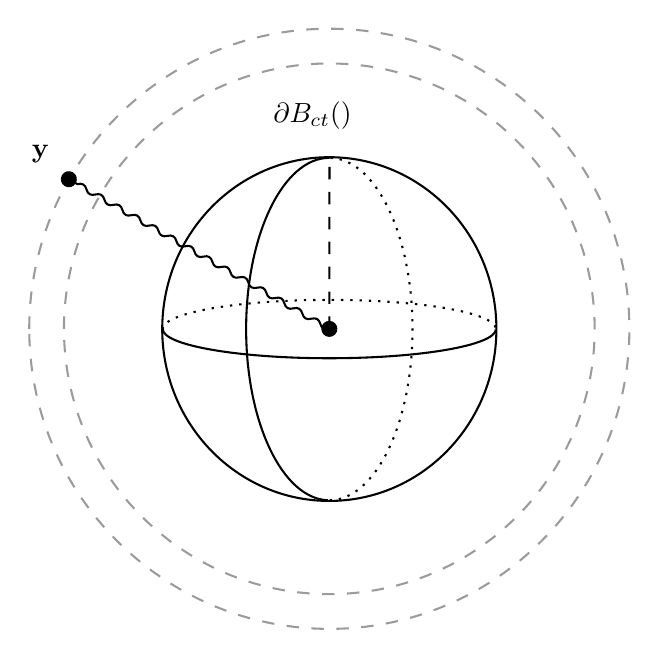
\begin{tikzpicture}[x=0.75pt,y=0.75pt,yscale=-1,xscale=1]
            %uncomment if require: \path (0,860); %set diagram left start at 0, and has height of 860

            %Shape: Arc [id:dp78123671281272] 
            \draw  [draw opacity=0][dash pattern={on 0.84pt off 2.51pt}] (271.06,418.72) .. controls (292.94,419.34) and (310.58,456.03) .. (310.58,501.2) .. controls (310.58,546.76) and (292.64,583.69) .. (270.5,583.69) .. controls (270.47,583.69) and (270.44,583.69) .. (270.41,583.69) -- (270.5,501.2) -- cycle ; \draw  [dash pattern={on 0.84pt off 2.51pt}] (271.06,418.72) .. controls (292.94,419.34) and (310.58,456.03) .. (310.58,501.2) .. controls (310.58,546.76) and (292.64,583.69) .. (270.5,583.69) .. controls (270.47,583.69) and (270.44,583.69) .. (270.41,583.69) ;
            %Shape: Arc [id:dp2264589440031377] 
            \draw  [draw opacity=0] (269.78,583.68) .. controls (247.98,582.89) and (230.42,546.27) .. (230.42,501.2) .. controls (230.42,455.65) and (248.36,418.71) .. (270.5,418.71) .. controls (270.53,418.71) and (270.56,418.71) .. (270.59,418.71) -- (270.5,501.2) -- cycle ; \draw   (269.78,583.68) .. controls (247.98,582.89) and (230.42,546.27) .. (230.42,501.2) .. controls (230.42,455.65) and (248.36,418.71) .. (270.5,418.71) .. controls (270.53,418.71) and (270.56,418.71) .. (270.59,418.71) ;
            %Straight Lines [id:da7611012286548011] 
            \draw  [dash pattern={on 4.5pt off 4.5pt}]  (270.5,501.12) -- (270.58,418.71) ;
            \draw [shift={(270.5,501.12)}, rotate = 270.06] [color={rgb, 255:red, 0; green, 0; blue, 0 }  ][fill={rgb, 255:red, 0; green, 0; blue, 0 }  ][line width=0.75]      (0, 0) circle [x radius= 3.35, y radius= 3.35]   ;
            %Shape: Ellipse [id:dp8873135089154796] 
            \draw   (190,501.2) .. controls (190,455.47) and (226.04,418.4) .. (270.5,418.4) .. controls (314.96,418.4) and (351,455.47) .. (351,501.2) .. controls (351,546.93) and (314.96,584.01) .. (270.5,584.01) .. controls (226.04,584.01) and (190,546.93) .. (190,501.2) -- cycle ;
            %Shape: Arc [id:dp7686939141018732] 
            \draw  [draw opacity=0][dash pattern={on 0.84pt off 2.51pt}] (190.23,501.39) .. controls (190.23,501.32) and (190.22,501.26) .. (190.22,501.2) .. controls (190.22,493.44) and (226.17,487.14) .. (270.5,487.14) .. controls (314.65,487.14) and (350.47,493.39) .. (350.77,501.11) -- (270.5,501.2) -- cycle ; \draw  [dash pattern={on 0.84pt off 2.51pt}] (190.23,501.39) .. controls (190.23,501.32) and (190.22,501.26) .. (190.22,501.2) .. controls (190.22,493.44) and (226.17,487.14) .. (270.5,487.14) .. controls (314.65,487.14) and (350.47,493.39) .. (350.77,501.11) ;
            %Shape: Arc [id:dp19047993718129197] 
            \draw  [draw opacity=0] (350.76,501.47) .. controls (349.95,509.11) and (314.33,515.26) .. (270.5,515.26) .. controls (226.43,515.26) and (190.66,509.04) .. (190.23,501.34) -- (270.5,501.2) -- cycle ; \draw   (350.76,501.47) .. controls (349.95,509.11) and (314.33,515.26) .. (270.5,515.26) .. controls (226.43,515.26) and (190.66,509.04) .. (190.23,501.34) ;
            %Shape: Ellipse [id:dp9844928716211963] 
            \draw  [color={rgb, 255:red, 155; green, 155; blue, 155 }  ,draw opacity=1 ][dash pattern={on 4.5pt off 4.5pt}] (142.66,501.07) .. controls (142.66,430.47) and (199.9,373.24) .. (270.5,373.24) .. controls (341.1,373.24) and (398.34,430.47) .. (398.34,501.07) .. controls (398.34,571.68) and (341.1,628.91) .. (270.5,628.91) .. controls (199.9,628.91) and (142.66,571.68) .. (142.66,501.07) -- cycle ;
            %Shape: Ellipse [id:dp32232142579971224] 
            \draw  [color={rgb, 255:red, 155; green, 155; blue, 155 }  ,draw opacity=1 ][dash pattern={on 4.5pt off 4.5pt}] (125.93,501.07) .. controls (125.93,421.23) and (190.65,356.5) .. (270.5,356.5) .. controls (350.35,356.5) and (415.07,421.23) .. (415.07,501.07) .. controls (415.07,580.92) and (350.35,645.65) .. (270.5,645.65) .. controls (190.65,645.65) and (125.93,580.92) .. (125.93,501.07) -- cycle ;
            %Straight Lines [id:da7905610574927917] 
            \draw    (270.5,501.2) .. controls (268.23,501.81) and (266.78,500.98) .. (266.17,498.71) .. controls (265.55,496.44) and (264.1,495.61) .. (261.83,496.22) .. controls (259.55,496.83) and (258.11,496) .. (257.5,493.72) .. controls (256.88,491.45) and (255.43,490.62) .. (253.16,491.23) .. controls (250.89,491.84) and (249.44,491.01) .. (248.83,488.74) .. controls (248.22,486.46) and (246.78,485.63) .. (244.5,486.24) .. controls (242.23,486.85) and (240.78,486.02) .. (240.16,483.75) .. controls (239.55,481.48) and (238.1,480.65) .. (235.83,481.26) .. controls (233.55,481.87) and (232.1,481.04) .. (231.49,478.76) .. controls (230.88,476.49) and (229.43,475.66) .. (227.16,476.27) .. controls (224.89,476.88) and (223.44,476.05) .. (222.83,473.78) .. controls (222.22,471.5) and (220.77,470.67) .. (218.49,471.28) .. controls (216.22,471.89) and (214.77,471.06) .. (214.16,468.79) .. controls (213.55,466.52) and (212.1,465.69) .. (209.83,466.3) .. controls (207.55,466.91) and (206.1,466.08) .. (205.49,463.8) .. controls (204.88,461.53) and (203.43,460.7) .. (201.16,461.31) .. controls (198.89,461.92) and (197.44,461.09) .. (196.82,458.82) .. controls (196.21,456.54) and (194.77,455.71) .. (192.49,456.32) .. controls (190.22,456.93) and (188.77,456.1) .. (188.16,453.83) .. controls (187.55,451.55) and (186.1,450.72) .. (183.82,451.33) .. controls (181.55,451.94) and (180.1,451.11) .. (179.49,448.84) .. controls (178.87,446.57) and (177.42,445.74) .. (175.15,446.35) .. controls (172.87,446.96) and (171.43,446.13) .. (170.82,443.85) .. controls (170.21,441.58) and (168.76,440.75) .. (166.49,441.36) .. controls (164.22,441.97) and (162.77,441.14) .. (162.15,438.87) .. controls (161.54,436.59) and (160.1,435.76) .. (157.82,436.37) .. controls (155.55,436.98) and (154.1,436.15) .. (153.48,433.88) .. controls (152.87,431.61) and (151.42,430.78) .. (149.15,431.39) -- (145,429) -- (145,429) ;
            \draw [shift={(145,429)}, rotate = 209.91] [color={rgb, 255:red, 0; green, 0; blue, 0 }  ][fill={rgb, 255:red, 0; green, 0; blue, 0 }  ][line width=0.75]      (0, 0) circle [x radius= 3.35, y radius= 3.35]   ;

            % Text Node
            \draw (272.27,488.72) node [anchor=north west][inner sep=0.75pt]    {$\x$};
            % Text Node
            \draw (242,390.33) node [anchor=north west][inner sep=0.75pt]    {$\partial B_{ct}(\x)$};
            % Text Node
            \draw (125.67,411) node [anchor=north west][inner sep=0.75pt]    {$\mathbf{y}$};

        \end{tikzpicture}

    \end{figure}
    \FloatBarrier

    al variare del tempo ho delle onde sferiche con supporto sul bordo della palla di centro $\x$ e raggio $ct$: un osservatore posto in $\y$ avvertirà la perturbazione solo all'istante:
    \begin{equation*}
        t=\frac{| \x -\y| }{c} ,
    \end{equation*}
    quindi:
    \begin{equation}
        \bigcup _{t >0} \partial B_{ct}(\x) =\partial C_{(\x ,0)}^{*}
    \end{equation}
    prende il nome di \textbf{cono caratteristico in avanti}, è il dominio di influenza del punto $\x$. Una conseguenza di quest'osservazione è che in dimensione $n=3$ esistono i \textbf{segnali sharp} (istantanei).
\end{oss}

\textbf{Passo 2}.

Sia $\displaystyle h=h(\x)$ qualunque. Scriviamo $h$ come sovrapposizione di impulsi:
\begin{equation*}
    ``\ h(\x) =\int _{\mathbb{R}^{3}} \delta _{3}(\x -\y) h(\y) \dyy \ "
\end{equation*}
o più formalmente:
\begin{equation*}
    \langle \delta _{3}(\x -\mathbf{\cdotp }) ,h\rangle =h(\x) .
\end{equation*}
Per il \textbf{Passo }$1$ a $\displaystyle \delta _{3}(\x -\y)$ corrisponde la soluzione:
\begin{equation*}
    K(\x ,\y ,t) =\frac{\delta (| \x -\y| -ct)}{4\pi c| \x -\y| } .
\end{equation*}
Se non uso un impulso unitario ma un impulso di intensità $\displaystyle h(\y)$ la soluzione diventa:
\begin{equation*}
    K(\x ,\y ,t) h(\y) .
\end{equation*}
Se uso $h$ espressa come somma di tutti gli impulsi mi basta fare l'integrale:
\begin{equation*}
    w_{h}(\x ,t) =\int _{\mathbb{R}^{3}} K(\x ,\y ,t) h(\y) \dyy =\int _{\mathbb{R}^{3}}\frac{\delta (| \x -\y| -ct)}{4\pi c| \x -\y| } h(\y) \dyy =(*)
\end{equation*}
passando in \textbf{coordinate polari} $\displaystyle (| \x -\y| =r)$ e usando una sorta di teorema di Fubini in coordinate polari:
\begin{equation*}
    (*) =\int _{0}^{+\infty }\frac{\delta (r-ct)}{4\pi cr} dr\int _{\partial B_{r}(\x)} h(\sigg) \dsig =(**)
\end{equation*}
\begin{oss}
    Ricordiamo che, per definizione della delta:
    \begin{equation}
        \int _{0}^{+\infty } \delta (r-ct) f(r) \dr=f(ct) .
        \label{eq:onde-osservazione-delta}
    \end{equation}
\end{oss}
Nel nostro caso possiamo scrivere:
\begin{equation*}
    (**) =\int _{0}^{+\infty } \delta (r-ct)\underbrace{\left[\frac{1}{4\pi cr}\int _{\partial B_{r}(\x)} h(\sigg) \dsig\right]}_{f(r)} \dr,
\end{equation*}
applicando la formula \eqref{eq:onde-osservazione-delta}\footnote{Il simbolo $\displaystyle \mint{-} $ indica il valor medio sulla superficie della sfera.}:
\begin{equation*}
    w_{h}(\x ,t) =\frac{1}{4\pi c^{2} t}\int _{\partial B_{ct}(\x)} h(\sigg) \dsig =t\underset{\partial B_{ct}(\x)}{\mint{-} } h(\sigg) \dsig .
\end{equation*}
\begin{theorem}
    [Formula di Kirchoff] Siano $\displaystyle g\in C^{3}\left(\mathbb{R}^{3}\right)$, $\displaystyle h\in C^{2}\left(\mathbb{R}^{3}\right)$. Allora:
    \begin{equation}
        u(\x ,t) =\frac{\partial }{\partial t}\left[\frac{1}{4\pi c^{2} t}\int _{\partial B_{ct}(\x)} g(\sigg) \dsig\right] +\frac{1}{4\pi c^{2} t}\int _{\partial B_{ct}(\x)} h(\sigg) \dsig
    \end{equation}
    è l'unica soluzione $\displaystyle u\in C^{2}\left(\mathbb{R}^{3} \times [ 0,+\infty)\right)$ del \eqref{eq:pcg-onde-3d}.
\end{theorem}
\begin{dimostrazione}
    Poiché $\displaystyle g\in C^{3}\left(\mathbb{R}^{3}\right)$ la funzione
    \begin{equation*}
        w_{g}(\x ,t) =\frac{1}{4\pi c^{2} t}\int _{\partial B_{ct}(\x)} g(\sigg) \dsig
    \end{equation*}
    soddisfa le ipotesi del Lemma A \vref{thm:lemma-A} e quindi è sufficiente controllare che
    \begin{equation*}
        w_{h}(\x ,t) =\frac{1}{4\pi c^{2} t}\int _{\partial B_{ct}(\x)} h(\sigg) \dsig
    \end{equation*}
    soddisfa l'equazione delle onde e le condizioni iniziali
    \begin{gather*}
        w_{h}(\x ,0) =0,\\
        \partial _{t} w_{h}(\x ,0) =h(\x) .
    \end{gather*}
    Notiamo che $\displaystyle h\in C^{2}\left(\mathbb{R}^{3}\right) \Rightarrow w_{h} \in C^{2}\left(\mathbb{R}^{3} \times [ 0,+\infty)\right)$.

    Effettuando il cambio di variabili
    \begin{equation*}
        \sigg =\x +ct\mathbf{w} ,\ \ \mathbf{w} \in \partial B_{1}(\zer) ,\dsig =c^{2} t^{2} d\mathbf{w}
    \end{equation*}
    possiamo scrivere
    \begin{equation*}
        w_{h}(\x ,t) =\frac{t}{4\pi }\int _{\partial B_{1}(\zer)} h(\x +ct\mathbf{w}) d\mathbf{w} .
    \end{equation*}
    Cominciamo coi dati iniziali
    \begin{align*}
        w_{h}(\x ,0)               & =0,                                                                                                                                                                                                                  \\
        \partial _{t} w_{h}(\x ,t) & =\frac{1}{4\pi }\int _{\partial B_{1}(\zer)} h(\x +ct\mathbf{w}) d\mathbf{w} +\textcolor[rgb]{0.82,0.01,0.11}{\frac{ct}{4\pi }\int _{\partial B_{1}(\zer)}\nabla h(\x +ct\mathbf{w})\cdotp \mathbf{w} d\mathbf{w} ,} \\
        \partial _{t} w_{h}(\x ,0) & =h(\x) .
    \end{align*}
    Per quanto riguarda l'equazione torniamo alle variabili originali:
    \begin{align*}
        \mathbf{w}                                                                                                                         & =\text{versore normale esterno}                                                                                                                                                                   &                          \\
        \textcolor[rgb]{0.82,0.01,0.11}{\frac{ct}{4\pi }\int _{\partial B_{1}(\zer)}\nabla h(\x+ct\mathbf{w})\cdotp \mathbf{w}d\mathbf{w}} & =\frac{1}{4\pi ct}\int _{\partial B_{1}(\zer)}\underbrace{\nabla h(\x +ct\mathbf{w})}_{\nabla h(\x +ct\mathbf{w}) =\nabla h(\sigg)} \cdotp \mathbf{w}\underbrace{c^{2} t^{2} d\mathbf{w}}_{\dsig} &                          \\
                                                                                                                                           & =\frac{1}{4\pi ct}\int _{\partial B_{ct}(\x)} \nabla h(\sigg) \cdotp \nuu \dsig                                                                                                                   &                          \\
                                                                                                                                           & =\frac{1}{4\pi ct}\int _{B_{ct}(\x)} \Delta h(\y) \dyy                                                                                                                                            & \text{(Teo. divergenza)} \\
                                                                                                                                           & =\frac{1}{4\pi ct}\int _{0}^{ct} dr\int _{\partial B_{r}} \Delta h(\sigg) \dsig ,                                                                                                                 & \text{(coord. polari)}
    \end{align*}
    quindi:
    \begin{equation*}
        \partial _{tt} w_{h}(\x ,t) =\cancel{\frac{c}{4\pi }\int _{\partial B_{1}(\zer)} \nabla h(\x +ct\mathbf{w}) \cdotp \mathbf{w} d\mathbf{w}} -\cancel{\frac{1}{4\pi ct^{2}}\int _{B_{ct}(\x)} \Delta h(\y) \dyy} +\frac{\cancel{c}}{4\pi \cancel{c} t}\int _{\partial B_{ct}(\x)} \Delta h(\sigg) \dsig ,
    \end{equation*}
    i primi due termini sono uguali (si vede svolgendo i passaggi di prima per tornare indietro), pertanto:
    \begin{equation*}
        \partial _{tt} w_{h}(\x ,t) =\frac{1}{4\pi t}\int _{\partial B_{ct}(\x)} \Delta h(\sigg) \dsig .
    \end{equation*}
    Calcoliamo il laplaciano di $\displaystyle w_{h}$:
    \begin{align*}
        \Delta w_{h}(\x ,t) & =\frac{t}{4\pi }\int _{\partial B_{1}(\zer)} \Delta h(\x +ct\mathbf{w}) d\mathbf{w} \\
                            & =\frac{1}{4\pi c^{2} t}\int _{\partial B_{ct}(\x)} \Delta h(\sigg) \dsig ,
    \end{align*}
    ma allora:
    \begin{equation*}
        \partial _{tt} w_{h} -c^{2} \Delta w_{h} =0.
    \end{equation*}
\end{dimostrazione}
\begin{oss}
    [In $\displaystyle \mathbb{R}^{3}$] Supponiamo di essere in $\x$ e interpretiamo $\displaystyle u(\x ,t)$ come perturbazione avvertita in $\x$ al tempo $t$:

    \begin{figure}[H]
        \centering

        \tikzset{every picture/.style={line width=0.75pt}} %set default line width to 0.75pt        

        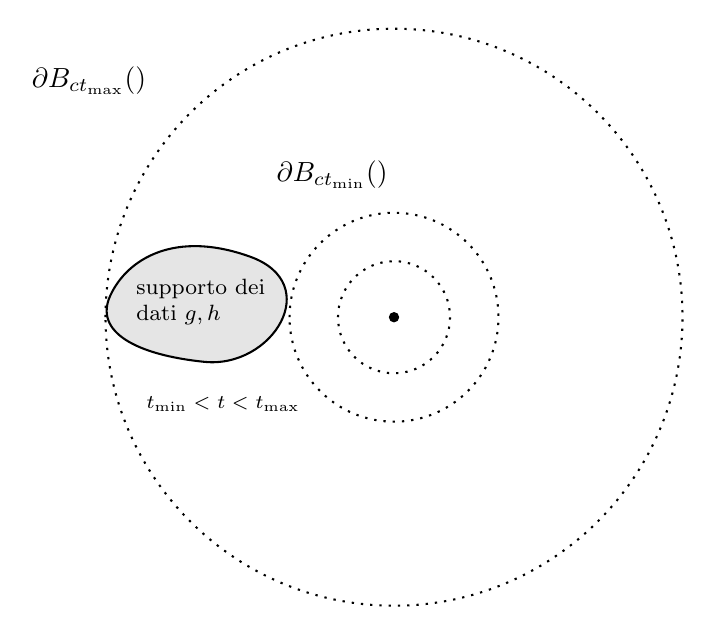
\begin{tikzpicture}[x=0.75pt,y=0.75pt,yscale=-1,xscale=1]
            %uncomment if require: \path (0,373); %set diagram left start at 0, and has height of 373

            %Shape: Polygon Curved [id:ds54562981881079] 
            \draw  [fill={rgb, 255:red, 0; green, 0; blue, 0 }  ,fill opacity=0.1 ] (126,149) .. controls (134.17,131.33) and (157.17,117.33) .. (193.33,130.33) .. controls (229.5,143.33) and (204,184.33) .. (171.33,181) .. controls (138.67,177.67) and (117.83,166.67) .. (126,149) -- cycle ;
            %Shape: Circle [id:dp07642569052374215] 
            \draw  [draw opacity=0][fill={rgb, 255:red, 0; green, 0; blue, 0 }  ,fill opacity=1 ] (260.17,159.5) .. controls (260.17,158.12) and (261.29,157) .. (262.67,157) .. controls (264.05,157) and (265.17,158.12) .. (265.17,159.5) .. controls (265.17,160.88) and (264.05,162) .. (262.67,162) .. controls (261.29,162) and (260.17,160.88) .. (260.17,159.5) -- cycle ;
            %Shape: Circle [id:dp48017364413518493] 
            \draw  [dash pattern={on 0.84pt off 2.51pt}] (235.67,159.5) .. controls (235.67,144.59) and (247.75,132.5) .. (262.67,132.5) .. controls (277.58,132.5) and (289.67,144.59) .. (289.67,159.5) .. controls (289.67,174.41) and (277.58,186.5) .. (262.67,186.5) .. controls (247.75,186.5) and (235.67,174.41) .. (235.67,159.5) -- cycle ;
            %Shape: Circle [id:dp9572432483506348] 
            \draw  [dash pattern={on 0.84pt off 2.51pt}] (212.33,159.5) .. controls (212.33,131.7) and (234.87,109.17) .. (262.67,109.17) .. controls (290.47,109.17) and (313,131.7) .. (313,159.5) .. controls (313,187.3) and (290.47,209.83) .. (262.67,209.83) .. controls (234.87,209.83) and (212.33,187.3) .. (212.33,159.5) -- cycle ;
            %Shape: Circle [id:dp5015811735444913] 
            \draw  [dash pattern={on 0.84pt off 2.51pt}] (123.67,159.5) .. controls (123.67,82.73) and (185.9,20.5) .. (262.67,20.5) .. controls (339.43,20.5) and (401.67,82.73) .. (401.67,159.5) .. controls (401.67,236.27) and (339.43,298.5) .. (262.67,298.5) .. controls (185.9,298.5) and (123.67,236.27) .. (123.67,159.5) -- cycle ;

            % Text Node
            \draw (141.83,196.23) node [anchor=north west][inner sep=0.75pt]  [font=\scriptsize]  {$t_{\min} < t< t_{\max}$};
            % Text Node
            \draw (257.33,137.73) node [anchor=north west][inner sep=0.75pt]    {$\x$};
            % Text Node
            \draw (86.67,37.4) node [anchor=north west][inner sep=0.75pt]    {$\partial B_{ct_{\max}}(\x)$};
            % Text Node
            \draw (204.67,82.73) node [anchor=north west][inner sep=0.75pt]    {$\partial B_{ct_{\min}}(\x)$};
            % Text Node
            \draw (137,139.67) node [anchor=north west][inner sep=0.75pt]  [font=\footnotesize] [align=left] {supporto dei\\dati $\displaystyle g,h$};

        \end{tikzpicture}
    \end{figure}
    \FloatBarrier

    La formula di Kirchoff ci dice che la perturbazione dipende dai valori di $g$ ed $h$ su $\displaystyle \partial B_{ct}(\x)$.

    Se $t$ è piccolo non avverto nulla, il tempo minimo per cui avvertirò la perturbazione sarà nell'istante $\displaystyle t_{\min}$ quando il bordo della sfera interseca per la prima volta il supporto, fino all'istante $\displaystyle t_{\max}$ oltre al quale non avvertirò più nulla. Questo fenomeno prende il nome di \textbf{principio di Huygens forte }(esistenza di segnali Sharp).
\end{oss}

\subsection{Caso \texorpdfstring{$n=2$}{n=2}}

Risolviamo il problema di Cauchy globale in dimensione $n=2$:
\begin{equation*}
    \tag{PCG$_{\text{onde,2D}}$}
    \begin{cases}
        u_{tt} -c^{2} \Delta u=0 & \x \in \mathbb{R}^{2} ,\ t >0,\ \x =
        \begin{pmatrix}
            x_{1} \\
            x_{2}
        \end{pmatrix}                                     \\
        u(\x ,0) =0              & \x\mathbb{\in R}^{2}                 \\
        u_{t}(\x ,0) =h(\x)      & \x\mathbb{\in R}^{2}
    \end{cases}
    \label{eq:pcg-onde-2d}
\end{equation*}
utilizzando il metodo della \textbf{discesa di Hadamard}: considero \eqref{eq:pcg-onde-2d} come un problema in dimensione $3$:
\begin{equation}
    (\x ,x_{3}) \in \mathbb{R}^{3} ,\ h(\x ,x_{3}) =h(\x)
\end{equation}
Cerco $\displaystyle w=w(\x ,x_{3})$ soluzione di
\begin{equation*}
    \begin{cases}
        w_{tt} -c^{2} \Delta _{3} w(\x ,x_{3}) =0 & \text{in} \ \mathbb{R}^{3} ,\ t >0 \\
        w(\x ,x_{3} ,0) =0                        &                                    \\
        w_{t}(\x ,x_{3} ,0) =h(\x)                &
    \end{cases}
\end{equation*}
questo problema lo so risolvere grazie alla formula di Kirchoff
\begin{equation*}
    w(\x ,x_{3} ,t) =\frac{1}{4\pi c^{2} t}\int _{\partial B_{ct}(\x ,x_{3})} h(\sigg) \dsig \dsig _{3} ,\ \ \sigg =(\sigma _{1} ,\sigma _{2})
\end{equation*}
devo far vedere che in realtà $\displaystyle w(\x ,x_{3}) =w(\x)$, cioè che non c'è reale dipendenza da $\displaystyle x_{3}$.

Osservo che la superficie sferica $\displaystyle \partial B_{ct}(\x ,x_{3})$ è unione dei due emisferi di equazione:
\begin{equation*}
    y_{3} =F_{\pm }(\y) =x_{3} \pm \sqrt{c^{2} t^{2} -r^{2}}
\end{equation*}
dove
\begin{equation*}
    r^{2} =| \x -\y| ^{2} =(x_{1} -y_{1})^{2} +(x_{2} -y_{2})^{2} .
\end{equation*}
Su entrambi gli emisferi $h$ non dipende da $\displaystyle x_{3}$, quindi abbiamo due integrali uguali. Inoltre possiamo riportare l'integrale sulla semi-superficie della sfera a un integrale doppio sul piano, a tutti gli effetti facendo una \textit{discesa}. Dal punto di vista dell'elemento infinitesimo la trasformazione è:
\begin{equation*}
    \dsig =\sqrt{1+| \nabla F_{\pm }(\y)| ^{2}} \dyy =\sqrt{1+\frac{r^{2}}{c^{2} t^{2} -r^{2}}} \dyy =\frac{ct}{\sqrt{c^{2} t^{2} -r^{2}}} \dyy,\qquad  (\dyy =\dy_{1} \dy_{2})
\end{equation*}
\begin{figure}[htpb]
    \centering


    \tikzset{every picture/.style={line width=0.75pt}} %set default line width to 0.75pt        

    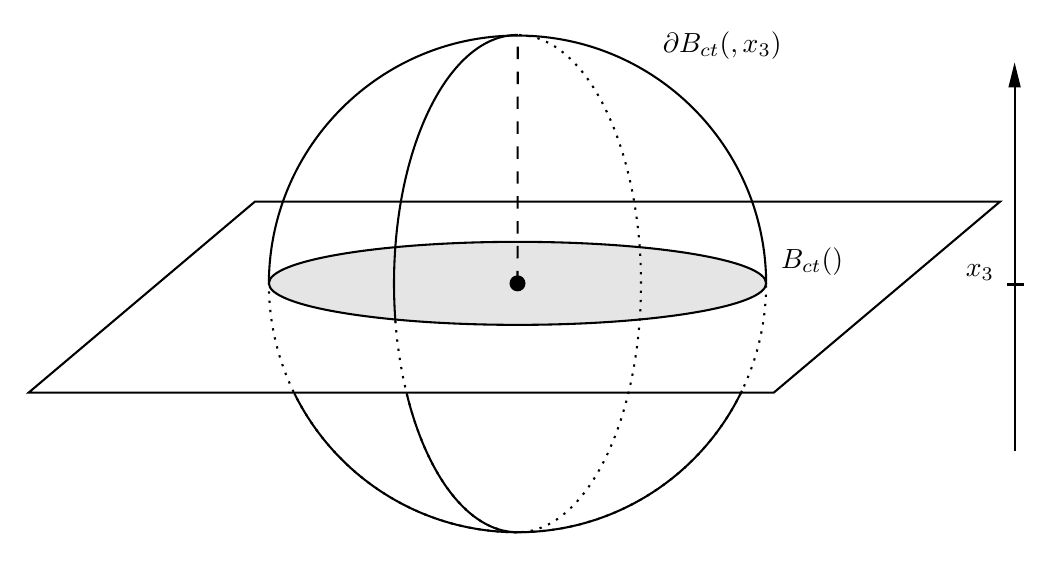
\begin{tikzpicture}[x=0.75pt,y=0.75pt,yscale=-1,xscale=1]
        %uncomment if require: \path (0,321); %set diagram left start at 0, and has height of 321

        %Shape: Parallelogram [id:dp20764399192874583] 
        \draw   (124,110.7) -- (483,110.7) -- (374,202.7) -- (15,202.7) -- cycle ;
        %Shape: Arc [id:dp670951507496512] 
        \draw  [draw opacity=0] (130.71,149.68) .. controls (131.14,83.9) and (184.61,30.7) .. (250.5,30.7) .. controls (316.66,30.7) and (370.3,84.34) .. (370.3,150.5) .. controls (370.3,150.54) and (370.3,150.58) .. (370.3,150.63) -- (250.5,150.5) -- cycle ; \draw   (130.71,149.68) .. controls (131.14,83.9) and (184.61,30.7) .. (250.5,30.7) .. controls (316.66,30.7) and (370.3,84.34) .. (370.3,150.5) .. controls (370.3,150.54) and (370.3,150.58) .. (370.3,150.63) ;
        %Shape: Arc [id:dp13700719688241492] 
        \draw  [draw opacity=0][dash pattern={on 0.84pt off 2.51pt}] (370.29,151.02) .. controls (369.86,216.81) and (316.39,270) .. (250.5,270) .. controls (184.34,270) and (130.7,216.37) .. (130.7,150.2) .. controls (130.7,150.16) and (130.7,150.12) .. (130.7,150.08) -- (250.5,150.2) -- cycle ; \draw  [dash pattern={on 0.84pt off 2.51pt}] (370.29,151.02) .. controls (369.86,216.81) and (316.39,270) .. (250.5,270) .. controls (184.34,270) and (130.7,216.37) .. (130.7,150.2) .. controls (130.7,150.16) and (130.7,150.12) .. (130.7,150.08) ;
        %Shape: Arc [id:dp713490243728391] 
        \draw  [draw opacity=0][dash pattern={on 0.84pt off 2.51pt}] (251.32,30.42) .. controls (283.8,31.3) and (310,84.59) .. (310,150.2) .. controls (310,216.37) and (283.36,270) .. (250.5,270) .. controls (250.46,270) and (250.42,270) .. (250.37,270) -- (250.5,150.2) -- cycle ; \draw  [dash pattern={on 0.84pt off 2.51pt}] (251.32,30.42) .. controls (283.8,31.3) and (310,84.59) .. (310,150.2) .. controls (310,216.37) and (283.36,270) .. (250.5,270) .. controls (250.46,270) and (250.42,270) .. (250.37,270) ;
        %Shape: Arc [id:dp5260933387102087] 
        \draw  [draw opacity=0] (191.71,168.78) .. controls (191.24,162.73) and (191,156.52) .. (191,150.2) .. controls (191,84.04) and (217.64,30.41) .. (250.5,30.41) .. controls (250.54,30.41) and (250.58,30.41) .. (250.63,30.41) -- (250.5,150.2) -- cycle ; \draw   (191.71,168.78) .. controls (191.24,162.73) and (191,156.52) .. (191,150.2) .. controls (191,84.04) and (217.64,30.41) .. (250.5,30.41) .. controls (250.54,30.41) and (250.58,30.41) .. (250.63,30.41) ;
        %Shape: Arc [id:dp21634156745075273] 
        \draw  [draw opacity=0][dash pattern={on 0.84pt off 2.51pt}] (249.85,269.99) .. controls (220.05,269.35) and (195.5,224.59) .. (191.55,166.61) -- (250.5,150.2) -- cycle ; \draw  [dash pattern={on 0.84pt off 2.51pt}] (249.85,269.99) .. controls (220.05,269.35) and (195.5,224.59) .. (191.55,166.61) ;
        %Shape: Ellipse [id:dp3396018229275308] 
        \draw  [fill={rgb, 255:red, 0; green, 0; blue, 0 }  ,fill opacity=0.1 ] (130.7,150.08) .. controls (130.7,139.03) and (184.34,130.08) .. (250.5,130.08) .. controls (316.66,130.08) and (370.3,139.03) .. (370.3,150.08) .. controls (370.3,161.12) and (316.66,170.08) .. (250.5,170.08) .. controls (184.34,170.08) and (130.7,161.12) .. (130.7,150.08) -- cycle ;
        %Straight Lines [id:da02584086910866268] 
        \draw  [dash pattern={on 4.5pt off 4.5pt}]  (250.5,150.08) -- (250.63,30.41) ;
        \draw [shift={(250.5,150.08)}, rotate = 270.06] [color={rgb, 255:red, 0; green, 0; blue, 0 }  ][fill={rgb, 255:red, 0; green, 0; blue, 0 }  ][line width=0.75]      (0, 0) circle [x radius= 3.35, y radius= 3.35]   ;
        %Straight Lines [id:da4742116163717902] 
        \draw    (490,230.7) -- (490,45.7) ;
        \draw [shift={(490,43.7)}, rotate = 450] [fill={rgb, 255:red, 0; green, 0; blue, 0 }  ][line width=0.08]  [draw opacity=0] (12,-3) -- (0,0) -- (12,3) -- cycle    ;
        %Straight Lines [id:da017887571875842445] 
        \draw    (494.3,150.63) -- (486.3,150.63) ;
        %Shape: Arc [id:dp20147168083416767] 
        \draw  [draw opacity=0] (358.62,201.85) .. controls (339.34,242.16) and (298.17,270) .. (250.5,270) .. controls (203.28,270) and (162.45,242.68) .. (142.93,202.99) -- (250.5,150.2) -- cycle ; \draw   (358.62,201.85) .. controls (339.34,242.16) and (298.17,270) .. (250.5,270) .. controls (203.28,270) and (162.45,242.68) .. (142.93,202.99) ;
        %Shape: Arc [id:dp5315503198873763] 
        \draw  [draw opacity=0] (249.85,269.99) .. controls (226.69,269.5) and (206.7,242.35) .. (197.09,203.07) -- (250.5,150.2) -- cycle ; \draw   (249.85,269.99) .. controls (226.69,269.5) and (206.7,242.35) .. (197.09,203.07) ;

        % Text Node
        \draw (376,131.4) node [anchor=north west][inner sep=0.75pt]    {$B_{ct}(\x)$};
        % Text Node
        \draw (259,140.4) node [anchor=north west][inner sep=0.75pt]    {$\x$};
        % Text Node
        \draw (319,27.4) node [anchor=north west][inner sep=0.75pt]    {$\partial B_{ct}(\x ,x_{3})$};
        % Text Node
        \draw (465,139.4) node [anchor=north west][inner sep=0.75pt]    {$x_{3}$};

    \end{tikzpicture}
    \caption{Discesa di Hadamard.}
\end{figure}
\FloatBarrier
quindi
\begin{equation*}
    w\left(\x ,\cancel{x_{3}} ,t\right) =\frac{1}{2\pi c}\int _{B_{ct}(\x)}\frac{h(\y)}{\sqrt{c^{2} t^{2} -| \x -\y| ^{2}}} \dyy
\end{equation*}
non dipende da $\displaystyle x_{3}$! Allora usando ancora una volta il Lemma A \vref{thm:lemma-A} otteniamo il seguente teorema.
\begin{theorem}
    [Formula di Poisson] Siano $\displaystyle g\in C^{3}\left(\mathbb{R}^{2}\right)$ e $\displaystyle h\in C^{2}\left(\mathbb{R}^{2}\right)$. Allora:
    \begin{equation}
        u(\x ,t) =\frac{1}{2\pi c}\left\{\frac{\partial }{\partial t}\int _{B_{ct}(\x)}\frac{g(\y)}{\sqrt{c^{2} t^{2} -| \x -\y| ^{2}}} \dyy +\ \int _{B_{ct}(\x)}\frac{h(\y)}{\sqrt{c^{2} t^{2} -| \x -\y| ^{2}}} \dyy\right\}
    \end{equation}
    è l'unica soluzione $\displaystyle \in C^{2}\left(\mathbb{R}^{2} \times [ 0,+\infty)\right)$ del \eqref{eq:pcg-onde-2d}.
\end{theorem}
Una differenza fondamentale è che gli integrali sono su tutta la sfera piena, non solo sulla superficie come in tre dimensioni: dopo $\displaystyle t_{\max}$ continuo a percepire la perturbazione. Di conseguenza \textit{il principio di Huygens forte non vale in dimensione }$2$ e non esistono segnali \textit{istantanei}.

Il fenomeno si può osservare ponendo un turacciolo in acqua calma e lasciando cadere un sasso poco distante. Il tappo rimane in quiete fino all'arrivo del primo fronte d'onda ma persiste nell'oscillazione anche dopo che questo è passato.